\documentclass[11pt,a4paper]{article}
\usepackage{fullpage}
\usepackage{amsmath}
\usepackage{amssymb}
\usepackage{amsfonts}
\usepackage{mathtools}
\usepackage{titlesec}
\usepackage{graphicx}
\usepackage{float}
\usepackage{wrapfig}
\usepackage{multicol}
\usepackage{caption}
\usepackage{hyperref}
\usepackage{apacite}
\usepackage{tabularx}
\usepackage{multirow}
\usepackage{subcaption}
\usepackage[noend]{algpseudocode}
\usepackage[nothing]{algorithm}
\usepackage{array}
\usepackage{xcolor}
\newcolumntype{T}{>{\tiny}l} % define a new column type for \tiny
\newcolumntype{H}{>{\Huge}l} % define a new column type for \Huge
\newcolumntype{P}[1]{>{\centering\arraybackslash}p{#1}}

\usepackage{stackengine}
\newsavebox\mybox
\newcommand\Includegraphics[2][]{\sbox{\mybox}{%
\includegraphics[#1]{#2}}\abovebaseline[-.5\ht\mybox]{%
\addstackgap{\usebox{\mybox}}}}

\algnewcommand\And{\textbf{and} }
\algnewcommand\Or{\textbf{or} }

\def\SPSB#1#2{\rlap{\textsuperscript{{#1}}}\SB{#2}}
\def\SP#1{\textsuperscript{{#1}}}
\def\SB#1{\textsubscript{{#1}}}


\DeclarePairedDelimiter{\ceil}{\lceil}{\rceil}
\DeclarePairedDelimiter\floor{\lfloor}{\rfloor}
\newcommand*{\field}[1]{\mathbb{#1}}%

\begin{document}  

\begin{titlepage} % Suppresses headers and footers on the title page

	\centering % Centre everything on the title page
	
	\scshape % Use small caps for all text on the title page
	
	\vspace*{\baselineskip} % White space at the top of the page
	
	%------------------------------------------------
	%	Title
	%------------------------------------------------
	
	
	\rule{\textwidth}{1.6pt}\vspace*{-\baselineskip}\vspace*{2pt} % Thick horizontal rule
	\rule{\textwidth}{0.4pt} % Thin horizontal rule
	
	\vspace{0.75\baselineskip} % Whitespace above the title
	
	{\LARGE Implementation and Analysis of Acceleration Data Structures in Ray tracing\\} % Title
	
	\vspace{0.75\baselineskip} % Whitespace below the title
	
	\rule{\textwidth}{0.4pt}\vspace*{-\baselineskip}\vspace{3.2pt} % Thin horizontal rule
	\rule{\textwidth}{1.6pt} % Thick horizontal rule
	
	\vspace{2\baselineskip} % Whitespace after the title block
	
	%------------------------------------------------
	%	Subtitle
	%------------------------------------------------
	
	Master Project Rendering Track \\ 
	SS 2022 % Subtitle or further description
	
	\vspace*{3\baselineskip} % Whitespace under the subtitle
	
	%------------------------------------------------
	%	Editor(s)
	%------------------------------------------------
	
	Written by
	
	\vspace{0.5\baselineskip} % Whitespace before the editors
	
	{\scshape\Large Alhajras Algdairy \\} % Editor list
	
			\vspace{0.5\baselineskip} % Whitespace before the editors

	Supervised by
	
	\vspace{0.5\baselineskip} % Whitespace before the editors
	
	{\scshape\Large Prof. Dr.-Ing. Matthias Teschner\\} % Editor list

	\vspace{0.5\baselineskip} % Whitespace before the editors
		
	\textit{Albert-Ludwigs-University of Freiburg \\ Chair of Computer Graphics} % Editor affiliation
	
		
\begin{figure}[h]	
     \centering
         
\includegraphics[width=3cm]{images/freiburg.png}
\end{figure}
	\vfill % Whitespace between editor names and publisher logo
	
	%------------------------------------------------
	%	Publisher
	%------------------------------------------------
	


	
	\vspace{0.3\baselineskip} % Whitespace under the publisher logo
	
	\today% Publication year
	

\end{titlepage}

\clearpage

\section*{Acknowledgements}
This project results from hard work and cumulative knowledge gained through seminars, labs, and lectures in the chair of Computer Graphics at the University of Freiburg under \textbf{Prof. Dr.-Ing. Matthias Teschner} guidness and supervision. Those materials and their resources were the fundamental building blocks to reaching this point with the proper feedback from the professor. The resources used in this project have been referenced and acknowledged wherever necessary.
\\
\section*{Abstract}
Improving the rendering time in a ray tracer is a challenging task. One of the improvement levels is to implement an acceleration data structure. There are two classifications of data structures namely, \textbf{spatial subdivision} and \textbf{object subdivision}. Both classifications are covered in the report. For object subdivision, \textbf{Bounding Volume Hierarchies (BVH)} and \textbf{Linear Bounding Volume Hierarchies (LBVH)} are implemented. For spatial subdivision, \textbf{Kd-Tree} is used. In this report, each method's strengths and weaknesses are explored by using different scenes and models.

\noindent
\\
\textbf{Keywords:} [BVH] [LBVH] [Kd-Tree] [ray tracing] [acceleration structure]  [object subdivision] [spatial
subdivision] 
\clearpage
\tableofcontents
\clearpage



\section{Introduction to Ray tracing}
\subsection{Overview}
Ray tracing is an algorithm that simulates how light behaves in a 3D scene to generate real-life digital images in a computer. This process is known as rendering. Rendering is used in various applications, such as Gaming, Animation, and Engineering.

\noindent
\\
Ray tracers have three different implementations, namely, Forward Ray tracing, Backward Ray tracing, and Hybrid Ray tracing. Regardless of which implementation is used, the general idea of the algorithm is straightforward but extremely powerful. It is to project the 3D scene into a 2D plane (Image). Firstly, a resolution must be chosen beforehand to divide the plane into small squares (Pixels). The next step is to evaluate the colour and illumination of each pixel. Several rays from the sensor (camera) toward the scene for each pixel are cast. Then it searches for any intersection by testing all the primitives, and if the ray hits one primitive, the primitive reference is saved into the hit list. Depending on the distance between the sensor and the hit primitive, the nearest primitives colour is returned. Shading is the next step; this includes knowing if the primitive is in a dark or bright region in the scene. This expensive process is recursively executed until the ray hits the light source or reaches a predefined depth. Testing the intersection is a performance challenge for thousands of primitives and more, as the process is linear in time.

\begin{figure}[h]	
     \centering
     \captionsetup{justification=centering,margin=2cm}
     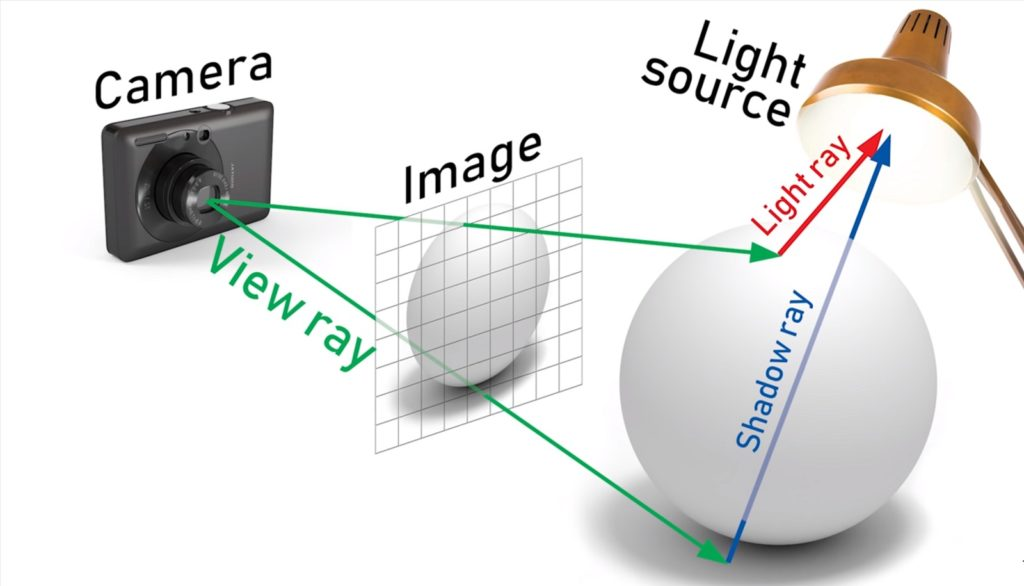
\includegraphics[width=8cm]{images/raytracer_2.jpg}
     \caption{A visual representation of ray tracing in which the rays are moving from the camera towards the scene. \protect\cite{Kimathi2020}}
     \label{fig:raytracer}
\end{figure}

\noindent
\\
Although the Rasterization method can render huge scenes relatively faster than ray tracers, Ray tracing algorithms can provide more photo-realistic images than rasterization, even though ray tracer consumes more time to render a scene. Accordingly, rasterization is used for real-time (online) applications such as gaming more than ray tracing; on the other hand, ray tracing is more often used in offline applications such as simulations and interior design software, where the lightning and shadow play an essential role to the output.
\clearpage

\begin{figure}[h]	
     \centering
     \captionsetup{justification=centering,margin=2cm}
     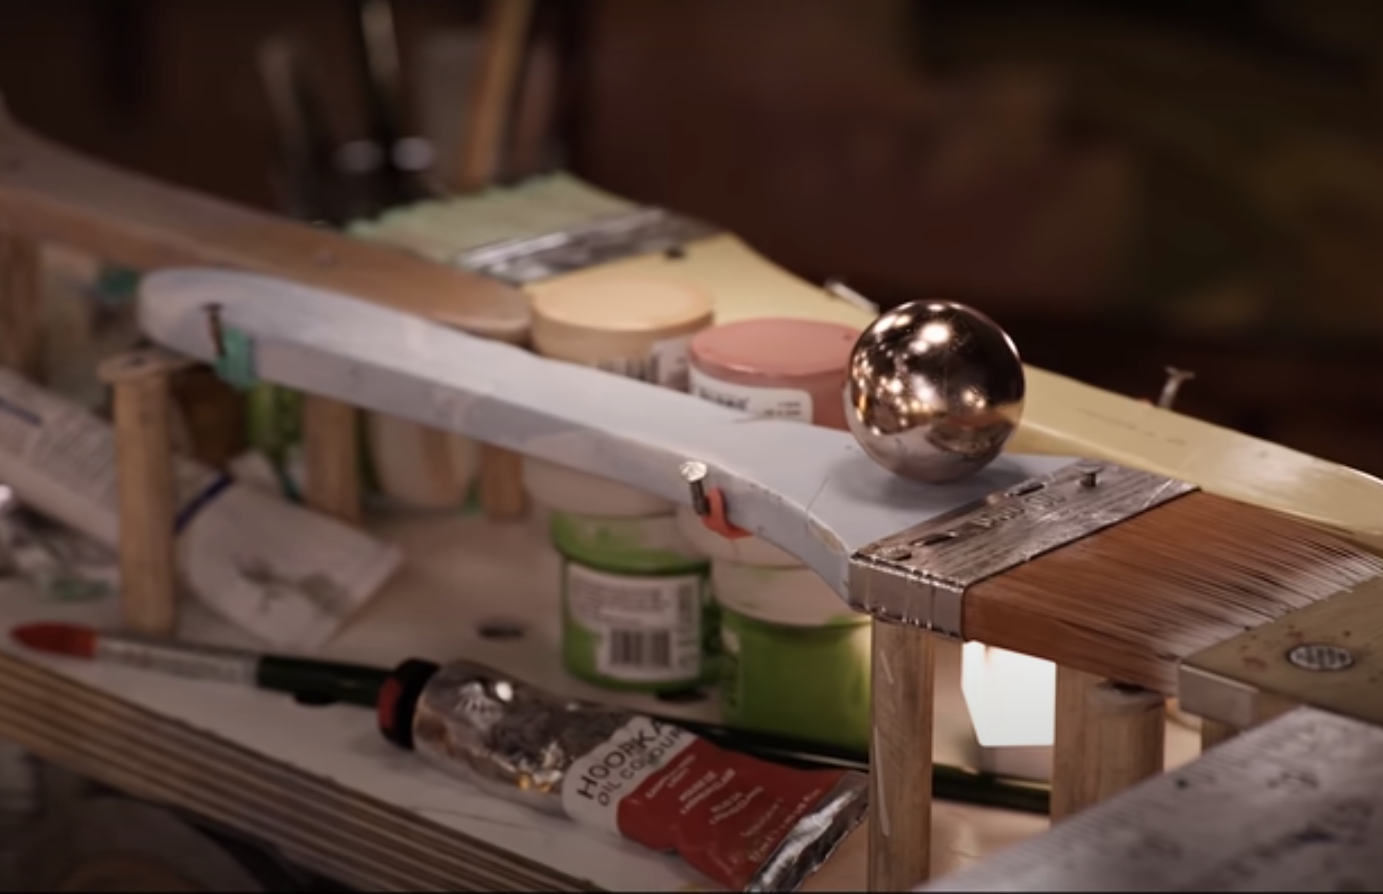
\includegraphics[width=10cm]{images/marbel_brush.png}
     \caption{NVIDIA RTX 3080 demo to realize real-time cinematic rendering.
\protect\cite{Burke2018}}
     \label{fig:rtxdemo}
\end{figure}

\noindent
\\
At Game Developers Conference, NVIDIA announced NVIDIA RTX™, a ray tracing technology that brings real-time gaming. The lighting, shadows, and surface reflection are so detailed in the marble scene that they look like a picture taken from a camera and not generated from a computer. The real challenge in real-time rendering is how to approximately render 60 high-quality frames per second.


\subsection{Motivation of using acceleration data structures}
In the ray tracing pipeline, we mentioned that each ray must execute an intersection test against all primitive contained in the scene. With $N$ number of pixels and $P$ number of primitives, this will produce a complexity of $\mathcal{O}(N.P)$. This is equivalent to a two-for-loop complexity $\mathcal{O}(n^2)$. Meaning for each pixel, even if it does not intersect with any primitive, we will have to perform an intersection test for all the primitives in the scene. The worst-case scenario is when the rays do not intersect with any primitive or model, but the ray tracer has to trace the rays in different directions still, resulting in an empty image. 

\noindent
\\
Brute forcing complexity is high; it increases linearly with the increase of the number of primitives. Moreover, some features such as anti-aliasing require more rays per pixel which increases the complexity to  $\mathcal{O}(N.P.S)$ where $S$ is the number of samples per pixel. 

\noindent
\\
Generally, using more samples will often produce a higher quality frame; additionally, for better illumination results, more recursion (Shadow rays) must be cast after each intersection. Hence, more rays are required for better quality but with fewer intersection tests as possible for better performance.

\noindent
\\
Giving a ray tracer that uses $S = 5$, $P = 100, 000$, and $N =  1, 280 $ x $1, 024$, $depth = 3$. This will give us a number of intersection tests, approximately $= 1, 280 * 1, 024 * 100, 000 * 5 * 3 = 1.96608*10^{12} $ intersection test. Assuming the machine used spends 0.01ms on each ray. This will result in 220 days of rendering one frame. Computers nowadays can handle this easily. However, the main challenge is scalability; some scenes contain millions of primitives making, rendering them by brute-forcing imposable.

\noindent
\\ 
Preprocessing algorithms to reorder and group the primitives to make them quickly traversed and tested can be used to overcome this challenge. \textbf{Spatial subdivision} and \textbf{object subdivision} are the two basic types of data acceleration structures. Spatial subdivision algorithms partition three-dimensional space into areas and keep track of which primitives overlap which regions. On the other hand, object subdivision algorithms gradually subdivide the scene's objects into smaller groups. This way, we can only test the primitives that have a higher probability of intersecting with the ray rather than testing all primitives that are not relevant to the region the ray passes through. 

\clearpage

\section{Bounding Volume Hierarchies (BVH)}
\subsection{Concept}
The basic idea of the BVH is simple yet powerful. It is to wrap all primitives in a virtual bounding box. This box will act as metadata to show the limits of the primitive and has no idea of how the shape of the primitive inside it. This concept will make it easier to test the primitives because one can wrap a complex model with one bounding box, and if the ray intersects the bounding box of the model, then and only then can we test its primitives.


\begin{figure}[h]	
     \centering
     \captionsetup{justification=centering,margin=2cm}
     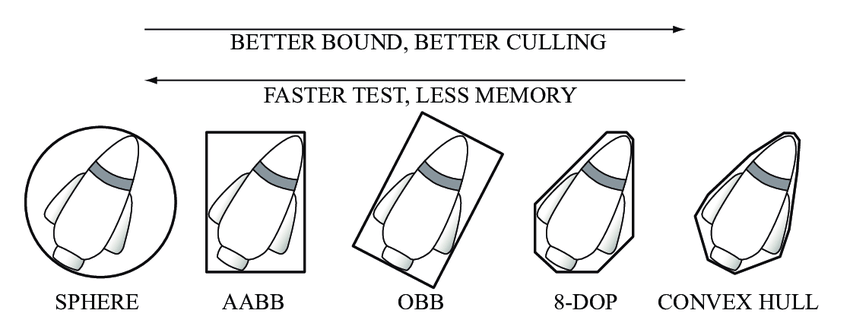
\includegraphics[width=10cm]{images/bvs.png}
     \caption{Bounding volumes: sphere, axis-aligned bounding box (AABB), oriented bounding box (OBB), eight-direction discrete orientation polytope (8-DOP), convex hull. \protect\cite{Ericson2004}}
     \label{fig:boundingboxes}
\end{figure}


\noindent
\\
The bounding volume can have different shapes, as shown in Figure ~\ref{fig:boundingboxes}. Although simple bounding volumes provide faster intersection tests, they often suffer from fitting to the model; eventually, they produce a large region of space. A compact bounding volume, on the other hand, generates fewer overlaps with other bounding volumes in the scene, producing fewer intersection tests. For example, spheres are probably the easiest bounding volume to generate for each primitive. Additionally, its intersection test is trivial and not expensive. However, we can note from the previous figure that it produces more empty regions that will be tested but will miss the model, eventually producing redundant tests. Using complex bounding volumes like \textbf{8-DOP} will have a higher probability of hitting the model and not missing it, but they are more difficult to generate and also more difficult to be tested. In this report, we will be using \textbf{AABB} because it is easy to implement, easy to test its intersection, and has less memory consumption because it only needs to save two 3D variables, the minimum and the maximum edges of the bounding box. One can use a combination of all of them, but in this report, we will only use the AABB.

\begin{figure}[h]	
     \centering
     \captionsetup{justification=centering,margin=2cm}
     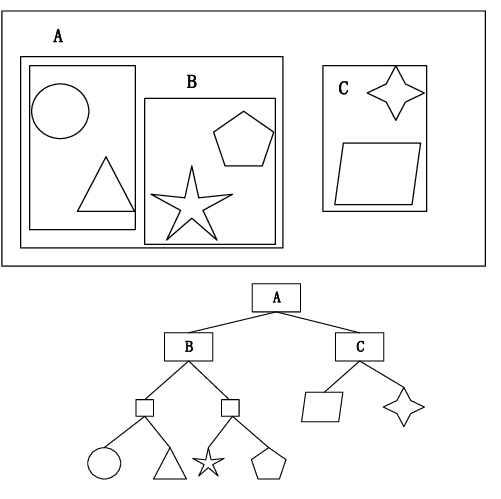
\includegraphics[width=8cm]{images/bvh_tree.png}
     \caption{BVH tree result by using AABB on a simple scene
. \protect\cite{Ericson2004} }
        \label{fig:boundingvolume}
\end{figure}

\noindent
\\
Figure ~\ref{fig:boundingboxes} shows a scene consists of six objects. Looking at the generated binary tree, we can note that every two objects are bounded by one AABB, and then each two AABB are joined and bounded by a bigger AABB. We recursively do this until we reach the root node that covers the limits of the whole scene. This will create a hierarchy of AABBs, and this is where the \textbf{Bounding Volume Hierarchies} name came from.

\noindent
\\
Without the BVH tree, we will have to go through all six objects for each ray intersection test, even for the rays that do not intersect with any object. On the other hand, when we introduced BVH, we can note that for the rays that do not even intersect with the root AABB node, we do not go further to test its children. This means we will only test once rather than six times. Looking at the sphere in Figure ~\ref{fig:boundingboxes}, if a ray intersects with it, we will only have to go through a path that goes $A \rightarrow B \rightarrow D \rightarrow Sphere$. These are four tests instead of six, and these four tests are the worst-case scenario as the longest path in the tree equals three. 

\noindent
\\
The worse case complexity for a binary tree is $\mathcal{O}(n)$, but if it is a balanced tree, it becomes $\mathcal{O}(\log{}n)$, this is significant, but the catch is we should try to build a balanced binary tree. This is where splitting criteria come in handy. 



\subsection{Implemntation}
BVH is made of two phases, Construction of the tree and Traversal over the tree.  

\subsubsection{Construction}
There are three methods to build the BVH binary tree: \textbf{Top-down}, \textbf{Bottom-up}, and \textbf{Insertion}. Top-down is arguably the most popular technique in practice. Hence this method will be implemented in this report. It uses the \textbf{fit \& split} algorithm, where it starts with the whole model and encapsulates it with a BV and fits it, then tries to split it
into n children, usually two. It keeps recursively splitting and fitting until it reaches the leaves and assigns the primitives to them.


\noindent
\\
Building a BVH tree needs predefined parameters. The depth of the tree, maximum allowed number of primitives in the leaf nodes, splitting axis, and bounding volume for wrapping primitives. The depth of the tree will not be predefined for the BVH tree. This means the tree can go deeper as possible. The maximum allowed primitives for each leaf will be chosen to be one. For bounding volume, as previously discussed, we will use only AABB. The splitting criteria and splitting axis will be discussed next.  
BVH tree can be constructed based on three different splitting criteria. There are four popular strategies to split the tree node:

\begin{itemize}
\item \textbf{Median of the centroid coordinates (Object median)}: The median of primitives, meaning if we have the next primitive positions in the x-axis as follows $\{1, 3, 3, 6, 7, 8, 9\}$ the median will be the primitive in the middle, which is $6$. This strategy will produce a well-balanced tree because it splits the primitives into two equal subtrees. Because this method is intuitive to implement and produces a well-balanced tree, this strategy will be adopted for the BVH tree. 

\item \textbf{Centroid method:}
This criteria focus on the bounding volume and not its primitives where it splits the AABB box into two half as follows:
\begin{equation}
\boldsymbol{c} = \frac{\boldsymbol{primitive_{AABB_{min}}}+\boldsymbol{primitive_{AABB_{max}}}}{2}
\end{equation}

\item  \textbf{Mean of centroid coordinates (Object mean)}: Using the mean of the primitives going back to the example $\{1, 3, 3, 6, 7, 8, 9\}$, the mean of this set is $5.2$, where the left child node will contain $\{1,3,3\}$ and the right child $\{6,7,8,9\}$

\item  \textbf{Spatial median}: Splitting the primitive's volume into two equal parts. For example, if we have four spheres with the next radius $\{1,1,1,4\}$, this strategy will split it as follow, the left child is $\{1,1,1\}$ and the right child is $\{4\}$ because it will split based on the volume/area of the sphere and not the position as the previous strategies. 


\end{itemize}


\begin{figure}[H]	
     \centering
     \captionsetup{justification=centering,margin=2cm}
     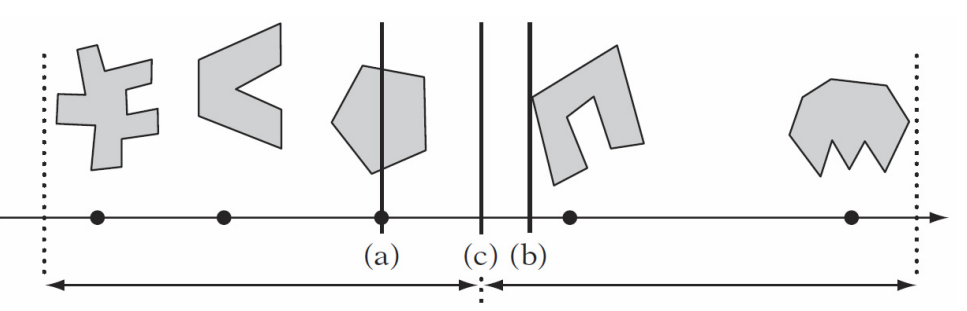
\includegraphics[width=10cm]{images/bvh_split.png}
     \caption{An example of (a) Object median splitting (b) Object mean splitting (c) Spatial median
splitting based on \protect\cite{Ericson2004}}
        \label{fig:dice}
\end{figure}

\noindent
\\
For choosing the splitting axis, one can use any axis, but this is a naive way to split. What happens if all primitives have the same z-axis and y-axis, but only the x-axis is changing, and we randomly choose to split by z-axis? This will usually produce an unbalanced tree. The optimal way is to calculate the longest axis for each node (AABB box). This way, we can try to split by the longest axis, which will produce a better-balanced tree. We can find the longest axis of the AABB box by using its diagonal $d$. 


\begin{equation}
\textbf{d} = \textbf{AABB}_{max} - \textbf{AABB}_{min}
\end{equation}

\noindent
\\
In Figure ~\ref{fig:aabbexample}, we have four spheres wrapped up by AABB. If we would like to choose one axis to split from, we can randomly start with the x-axis. As it is illustrated, choosing this axis will not give us a middle point to split point since all spheres have the same x-axis. Same for the y-axis. On the other hand, we can see that the Z-axis will split the AABB box into two AABB boxes, each containing two spheres. Again we can rechoose the z-axis to split those two AABB boxes. Finding the longest diagonal will indicate the largest spreading direction of the primitives in the scene. After finding $d$, we find the maximum axis of the diagonal as the next splitting axis.

\begin{figure}[H]	
     \centering
     \begin{subfigure}[t]{0.3\textwidth}
         \centering
         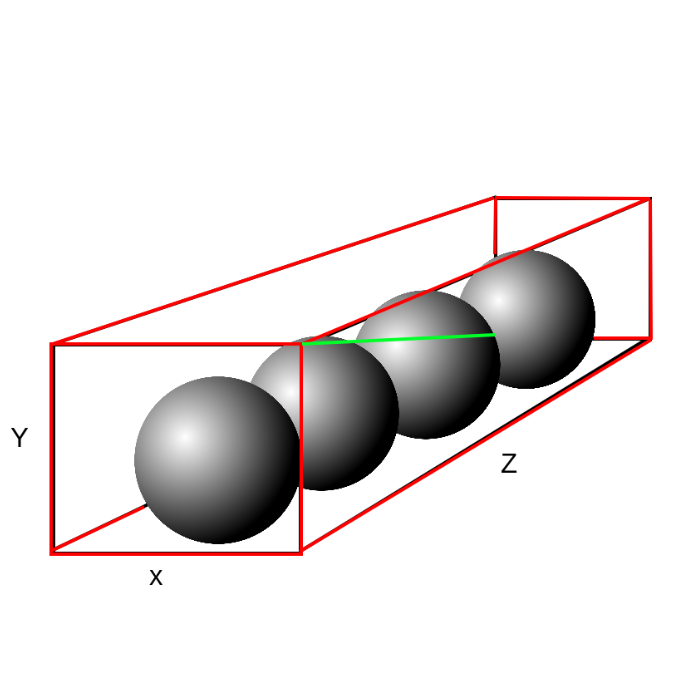
\includegraphics[width=\textwidth]{images/longaxis.png}
         \caption{}
         \label{fig:pi_4000}
     \end{subfigure}
     \hfill
     \begin{subfigure}[t]{0.3\textwidth}
         \centering
         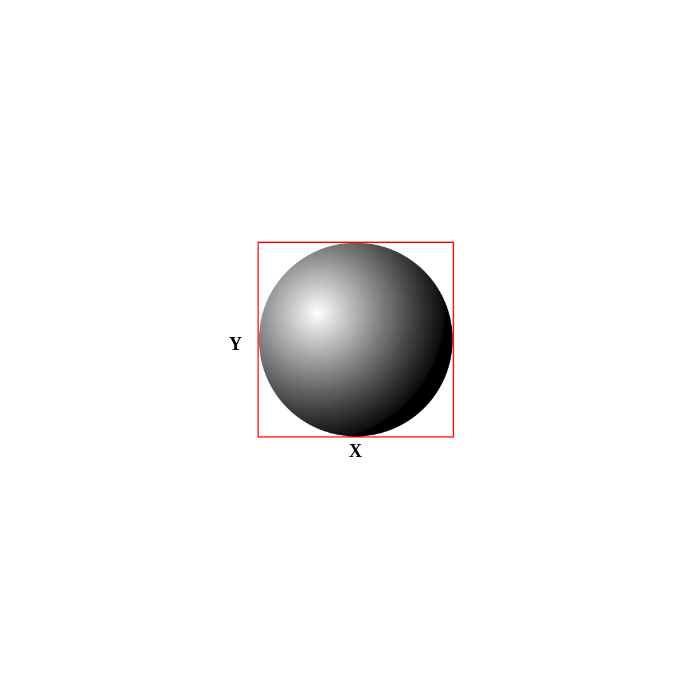
\includegraphics[width=\textwidth]{images/LONGAXIS_Y.png}
         \caption{}
         \label{fig:pi_5000}
     \end{subfigure}
     \hfill
     \begin{subfigure}[t]{0.3\textwidth}
         \centering
         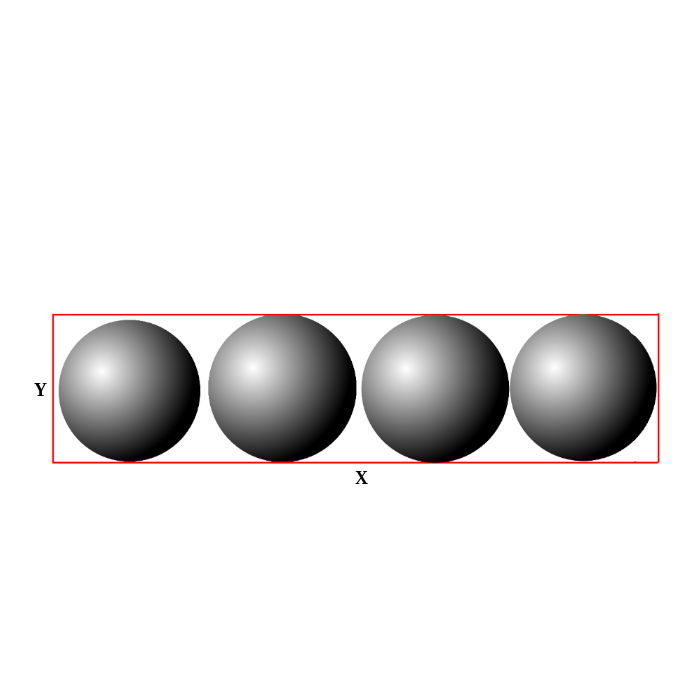
\includegraphics[width=\textwidth]{images/LONGAXIS_Z.png}
         \caption{}
         \label{fig:pi_18000}
     \end{subfigure}
        \captionsetup{justification=centering,margin=2cm}
        \caption{(a) Finding the diagonal of the AABB box is shown in green. (b) Vertical view of the scene where choosing either x-axis or y-axis will not make a difference. (c) Horizontal view of the scene where the z-axis makes the perfect splitting axis due to its wide distribution.}
        \label{fig:aabbexample}
\end{figure}

\subsubsection{Visual Illustration}
For a better illustration of how to build the BVH tree by using the centroid coordinates splitting criteria and also by choosing the longest axis to split from, we will look at the next scene as an example: 

\begin{figure}[h]	
     \centering
     \begin{subfigure}[t]{0.3\textwidth}
         \centering
         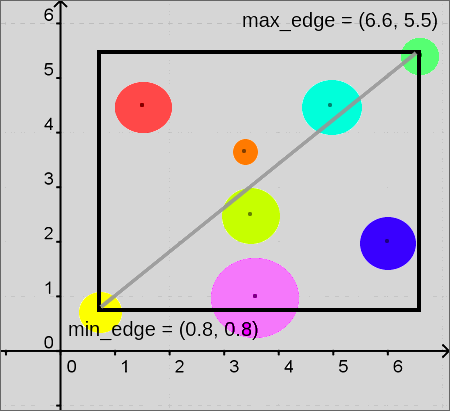
\includegraphics[width=\textwidth]{images/example_bvh/2_g.png}
         \captionsetup{justification=centering,margin=0.1cm}
         \caption{Root node and its AABB (Black) that covers all primitives and it's diagonal (Gray).}
         \label{fig:pi_4000}
     \end{subfigure}
     \hfill
     \begin{subfigure}[t]{0.3\textwidth}
         \centering
         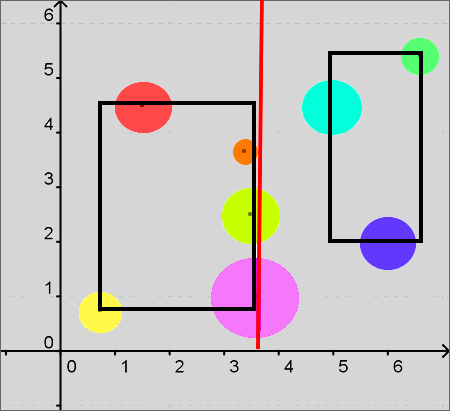
\includegraphics[width=\textwidth]{images/example_bvh/3_g.png}
         \captionsetup{justification=centering,margin=0.1cm}
         \caption{The second level in the tree splits the primitives into two groups by creating two internal nodes.}
         \label{fig:pi_5000}
     \end{subfigure}
     \hfill
     \begin{subfigure}[t]{0.3\textwidth}
         \centering
         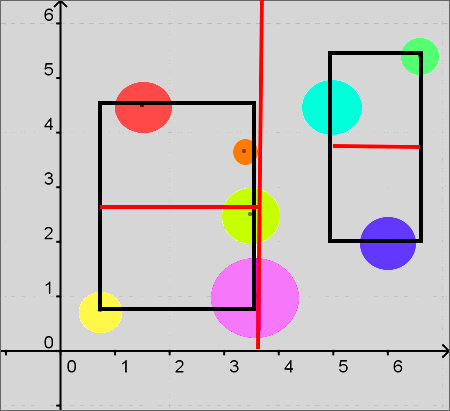
\includegraphics[width=\textwidth]{images/example_bvh/4_g.png}
         \captionsetup{justification=centering,margin=0.1cm}
         \caption{The third level in the tree splits the primitives into four groups, creating three internal nodes and a leaf node.}
         \label{fig:pi_18000}
     \end{subfigure}
        \captionsetup{justification=centering,margin=2cm}
        \caption{Building a BVH tree from top to bottom (root to leaves). Wrapping AABBs and splitting them into two halves recursively until reaching leaves.}
        \label{fig:three graphs}
\end{figure}

\noindent
\\
Since the Top-down approach is chosen, we will start creating the nodes from top to bottom. Firstly, we start creating the root node. Each node needs to save the AABB bounds ($minimum\_edge$, $maximum\_edge$), the splitting point, and the splitting axis. If the node is a leaf node, we will save the assigned primitives ids. We can calculate the $minimum\_edge$ (the minimum 3D point in our root AABB) and the $maximum\_edge$ point (the maximum 3D point in the AABB box) by easily iterating through all primitives in the scene and assigning the minimum primitive centroid to the  $minimum\_edge$ and the maximum primitive centroid to the $maximum\_edge$. The final result is $maximum\_edge = (6.6, 5.5)$ and  $minimum\_edge = (0.8,0.8)$.

\noindent
\\
After creating the root AABB, the second step is to find the splitting point by using the AABB boundaries. As we mentioned, we will find the longest axis first. To find the longest axis, we have to calculate the diagonal $d$ by subtracting the $minimum\_edge$ from $maximum\_edge $ and finding the maximum of both axes $max(maximum\_edge - minimum\_edge)$. This will give us $max((6.6-0.8) , (5.5-0.8)) = max(5.8,4.7) = 5.8$, which corresponds to the x-axis. 

\noindent
\\
Now we calculate the splitting point by just halfing the distance between $maximum\_edge $ and the $minimum\_edge$, $split\_point = \frac{0.8+6.6}{2} = 3.6$.

\noindent
\\
Then we pass all primitives that have a centroid $ < 3.6$ to the left child node, and we pass the rest to the right child node.  

\noindent
\\
Recustivly we keep doing this until the number of primitives in the node is less than the maximum allowed number of primitives parameter, which in this implementation, we decided to set to $1$. Then we create a leaf node that holds this primitive id. 


\begin{figure}[h]	
     \centering
     \captionsetup{justification=centering,margin=2cm}
     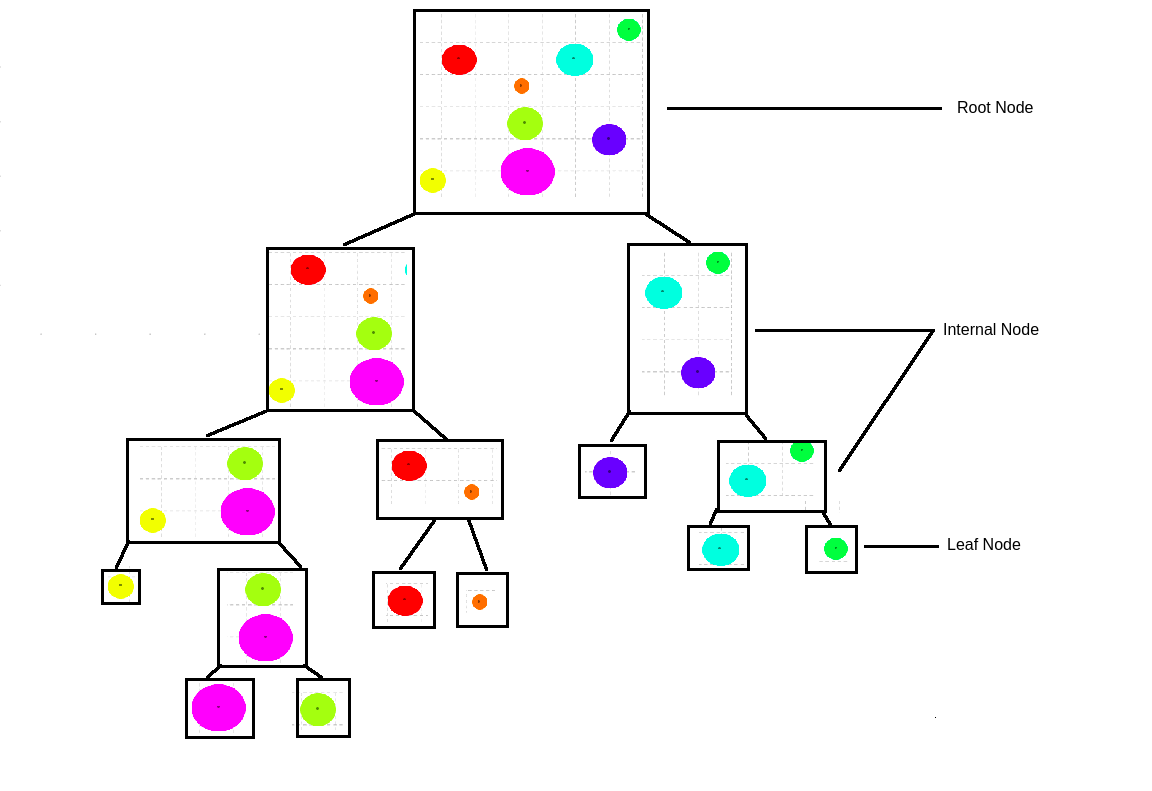
\includegraphics[width=9cm]{images/example_bvh/tree.png}
     \caption{The generated BVH tree by using centroid splitting criteria and AABB as BV.}
     \label{fig:dice}
\end{figure}

\subsubsection{Traversal}
The traversal phase of BVH is quite intuitive if you are familiar with how binary tree traversal works. After building the BVH tree, we start with its root node, we get its AABB boundaries, and we test its intersection with the ray. If the ray intersects with the AABB, we go to its left and right children and do the same process; otherwise, we terminate. Recursively keep doing this until we reach a leaf node; the leaf node is the node that has no node children, and it is the only node that contains a primitive inside it. Then we go through the list of primitives and test each one if it intersected with the ray or not. Remember that since we are using one primitive for each leaf node, the primitive's list will only contain one primitive, and this will not create a linear performance burden. 

\noindent
\\
As discussed, the leaf node can include a list of primitives and not only one by setting a parameter called $max\_leaf\_premitives$ to 1; this depends on how you configure the BVH building tree method. In this report, I set the list to make it only contain one primitive. It is worth noticing that the bigger $max\_leaf\_premitives$ is, the smaller the depth of the tree becomes because we do not have to keep splitting until we reach a leaf that only contains primitives less or equal to $max\_leaf\_premitives$. Therefore, less traversal time and less memory consumption because of the number of nodes saved. On the other hand, this will lead to a long list of primitives inside the leaf node, adding a linear time complexity for iterating through all the lists, which kills the purpose of using the hierarchy of the BVH to make the complexity logarithmic.


\noindent
\\
The intersection test is split into two main steps. First, we go through all the nodes in the tree, and if we hit a leaf node, we add all its primitives into a list called $hitList$. The $hitList$ list acts as a candidate list of the primitives that might intersect with the ray. Afterwards, we go through these candidates and find which are intersected and which one is the nearest to the camera by comparing the intersecting point distance to the camera centre position.

\begin{algorithm}[H]
	\caption{$intersectBVH$}\label{alg:alg1}
	\begin{algorithmic}
		\Require $ray$, $node$, $hitList$
		\If{$node$ $\rightarrow$ $boxIntersect(ray) = false $}
			\State $return\;\;false$
		\EndIf
		\If{$node$ $\rightarrow$ $isleaf$}
		    \State $hitList$ $\rightarrow$ $push(node \rightarrow premitives)$
		\Else
			\State $intersectBVH(ray, node \rightarrow leftChild,\, hitList)$
			\State $intersectBVH(ray, node \rightarrow rightChild,\, hitList)$
		\EndIf
	\end{algorithmic}
\end{algorithm}

\clearpage

\section{Linear Bounding Volume Hierarchies (LBVH)}
\subsection{Concept}
While BVH boosts the renderer's performance and makes it possible to render millions of primitives in minutes, it introduces an extra step in the rendering pipeline, which is a preprocess for building the tree. The building tree process can take half of the rendering time; nevertheless, creating this tree will make the render faster to find the intersected primitive. The question now is, can we do something about it? 

\noindent
\\
One way to solve this is to parallelize the building process. The parallelization can be done if the subtrees are independent of each other. This is what Linear Bounding Volume Hierarchies do. It creates a subprocess to make them build sub trees and join them at the end of the building of the subtrees to make one node. Naturally, parallelization will boost the performance of the construction time. Hence we will not compare it with the normal BVH. However, we will treat the LBVH as different splitting criteria and compare its performance with the BVH.

\noindent
\\
The first step is transforming the building tree problem into a sorting problem. We map the 3D centroid points for each primitive to one value that can be sorted. Morton codes do this mapping. Morton code map multidimensional data to one dimension while preserving the locality of the data points \protect\cite{wikipedia2022}. The transformation is done by interleaving the bits of the primitive's centroid in base 2. for example, taking a 3D point (x,y,z), the result Morton code will be calculated as follows: 
 
\begin{equation}
 ...z_3y_3x_3z_2y_2x_2z_1y_1x_1z_0y_0x_0
\end{equation}

\begin{align*}
& p_x = \textcolor{brown}{1010}, \;p_y = \textcolor{red}{0111}, \;p_z = \textcolor{blue}{1100} \\
&Morton\;code = \textcolor{blue}{1}\textcolor{red}{0}\textcolor{brown}{1} \;\textcolor{blue}{1}\textcolor{red}{1}\textcolor{brown}{0} \;\textcolor{blue}{0}\textcolor{red}{1}\textcolor{brown}{1} \;\textcolor{blue}{0}\textcolor{red}{1}\textcolor{brown}{0}
\end{align*}

\noindent
\\
After mapping the 3D point to 1D Morton code, we can use a sorting algorithm as a Radix sort \protect\cite{Karras2012}.

\subsubsection{Morton Code as a Splitting Criteria}
After mapping all primitives centroid to a Morton code and sorting them, the next step is knowing how to use the sorted list to build the tree. To better understand how the LBVH constructs the binary tree, we will illustrate this with a scene as shown in Figure ~\ref{fig:mortonexample}
. The scene is made out of 16 primitives distributed as shown. The first step is to generate the Morton code for each centroid point. Looking closely into the generated Morton codes of each primitive, we can note that each bit acts as a splitting plane that splits the primitives into more than one region. 

\noindent
\\
The first bit will split the y-axis into two regions. The first region with the first bit equals $1$, and the second region with the first bit equals $0$. For the binary tree, we can assign primitives with the zeros $0$xxx on the left child and the primitives with ones $1$xxx on the right. The second bit will split the scene into two areas by an x-axis plane. The third bit will split the y-axis into four regions.


\begin{figure}[H]	
     \centering
     \begin{subfigure}[b]{0.475\textwidth}
         \centering
         \captionsetup{justification=centering}
         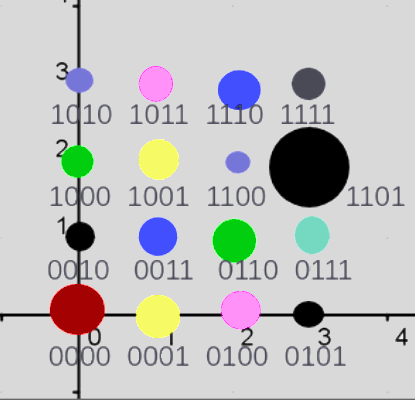
\includegraphics[width=5cm]{images/example_lbvh/morton_g.png}
         \caption{}
         \label{fig:pi_4000}
     \end{subfigure}
     \hfill
     \begin{subfigure}[b]{0.475\textwidth}
         \centering
         \captionsetup{justification=centering}
         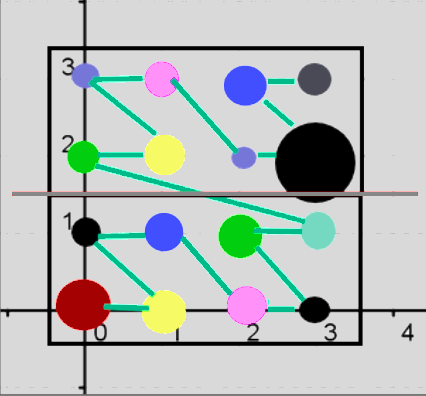
\includegraphics[width=5cm]{images/example_lbvh/01_g.png}
         \caption{}
         \label{fig:pi_5000}
     \end{subfigure}
     \hfill
     \begin{subfigure}[b]{0.475\textwidth}
         \centering
         \captionsetup{justification=centering}
         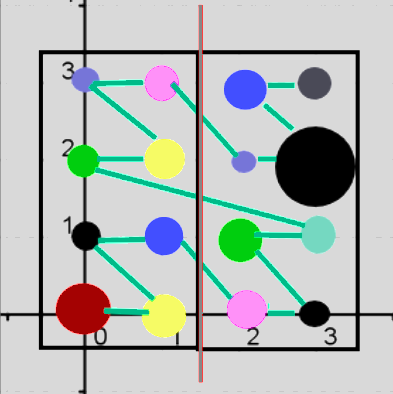
\includegraphics[width=5cm]{images/example_lbvh/02_g.png}
         \caption{}
         \label{fig:pi_18000}
     \end{subfigure}
        \captionsetup{justification=centering,margin=2cm}
             \hfill
     \begin{subfigure}[b]{0.475\textwidth}
         \centering
         \captionsetup{justification=centering}
         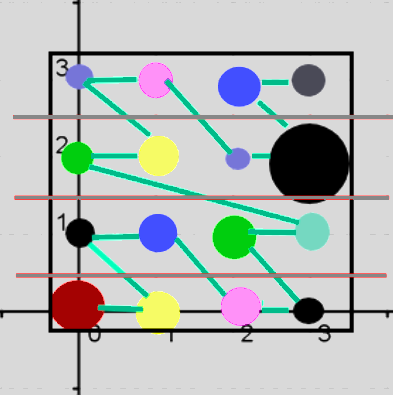
\includegraphics[width=5cm]{images/example_lbvh/03_g.png}
         \caption{}
         \label{fig:pi_18000}
     \end{subfigure}
        \captionsetup{justification=centering,margin=2cm}

        \caption{(a) The generated Morton code for 2D primitive's centroids. (b) The first splitting plane splits on the y-axis. (c) Second-highest bit of the Morton code splits the x-axis in the middle. (d) The third bit splits the primitives into four regions. }
        \label{fig:mortonexample}
\end{figure}



\begin{figure}[h]	
     \centering
     \captionsetup{justification=centering,margin=2cm}
     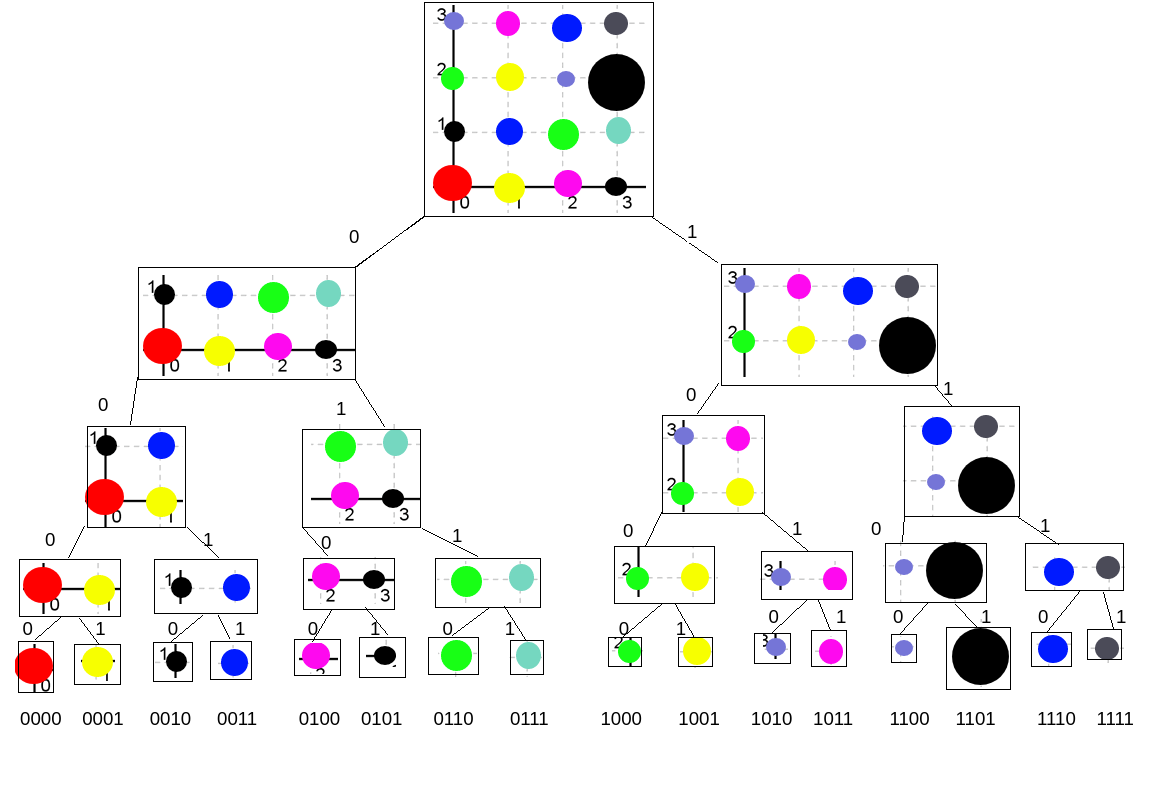
\includegraphics[width=12cm]{images/example_lbvh/tree.png}
     \caption{Generated tree by LBVH.}
     \label{fig:dice}
\end{figure}


\subsection{Implemntation}
The implementation includes two essential stages, Constructing the tree and tree Traversal. Traversal will not be repeated since the produced tree is a binary tree similar to the BVH. Hence the same traversal algorithm used in the BVH will be utilized for LBVH. Nevertheless, the main focus of the LBVH is building the tree.


\subsubsection{Construction}
The first step is to generate the Morton code for each primitive and to save time. One can generate the Morton code for each primitive and start sorting them while reading the primitives from the scene. It is better than reading the whole scene than going through all primitive in linear time and then sorting them by Radix sort.

\noindent
\\
Next, we create the nodes and split them based on the leading bits. We start with the sorted Morton code and search for the first leading bit change. Once the bit flips, we assign the zeros to the left child node and the rest to the right child node. We calculate the global bounding box for the current primitives and create the current node since we have all we need, an AABB box and a splitting point. We recursively keep doing this until we reach leaves and assign the primitives indexes or ids to the leaves. Remember, we use an unlimited depth for the LBVH. Also, the maximum number of primitives in a leaf was set to one.

\noindent
\\
Until this point, LBVH acts as a splitting criterion of a BVH. As we discussed, LBVH makes it trivial to parallelize the construction stage. To achieve this, we will use a simple conditional multithreading mechanism. Building the tree will only create a new thread if the number of primitives in the subtree is more than 100 primitives. Note that this is a random number chosen, but we do not want to create a new thread for small subtrees because it is not worth it. Note that for a fair comparison between the data structures, we will not parallelize LBVH and will only run it on one thread. 


\begin{algorithm}[H]
\caption{$constructLBVH$}\label{alg:alg1}
\begin{algorithmic}
		\Require $allPrimitives$, $sortedMortonCodes$, $startI$, $endI$
\State $node$ $\gets$ $createNewNode()$
\State $increaseTotalNumberOfNodes()$

\State $aabb$ $\gets$ $getGlobalAABB(primitives)$
\State $primitives$ $\gets$  $endI$ - $startI$
\If{$primitives = 0$}
	\State $node \rightarrow isleaf \gets true$
	\State $node \rightarrow prims \gets allPrimitives[startI]$
	\State \Return $node$
\EndIf

\State $split \gets findSplitPoint(sortedMortonCodes, startIndex, endIndex)$
\State $node \rightarrow leftchild  \gets constructLBVH(allPrimitives, startI, split)$
\State $node \rightarrow rightchild  \gets constructLBVH(allPrimitives, split, endI)$
\State \Return $node$
\end{algorithmic}
\end{algorithm}
\clearpage



\section{K Dimensional Tree (Kd-Tree)}
\subsection{Concept}
Two accelerator data structures, the BVH and LBVH, are already covered. Both methods are of type object subdivision. This chapter will discuss and implement a different accelerator called Kd-Tree, a spatial subdivision type. Kd-Tree is a traditional data structure that organizes K-dimensional points into a binary tree for easy retrieval. Unlike a typical binary tree, the Kd-Tree can have several dimensions at each level. It has been frequently utilized in multidimensional crucial data search because it effectively resolves multidimensional searching issues such as performance. In rendering applications, 3D dimension is used, and Kd-Tree can also be used.

\noindent
\\
The main idea is to divide the scene into regions. Each region will contain a list of primitives that intersect it. When we start rendering and start the intersection tests, we start looking for areas that intersect with the ray, and if we find an intersection, we only test the primitives that fall in it. The following Figure ~\ref{fig:kdtreedemo} gives an overview of how the spaces are divided:


\begin{figure}[h]	
     \centering
     \captionsetup{justification=centering,margin=2cm}
     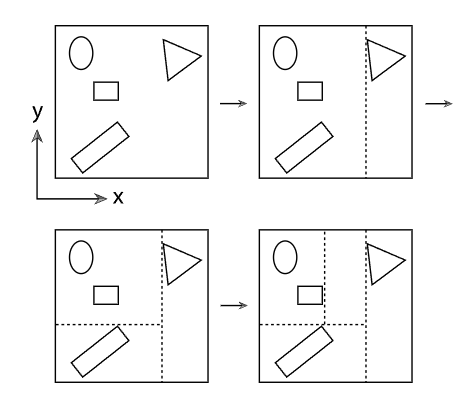
\includegraphics[width=10cm]{images/kdtree/example_demo.png}
     \caption{The Kd-Tree is built by splitting the scene into four regions where one axis is chosen with a splitting point for each split.  The first split is done on the x-axis, then the y-axis and the last split is on the x-axis again. \protect\cite{Pharr2016}}
        \label{fig:kdtreedemo}
\end{figure}



\subsubsection{Compact tree representation}
Unlike what we did in the BVH, the representation of the Kd-Tree will be compact. This means that rather than saving two children pointers left and right to the node, we will save all nodes in an array, where the left child lives right after the parent node in the array, and the right child node can be reached by saving the offset. Doing so improves cache, memory, and thus overall system performance.


\begin{figure}[h]	
     \centering
     \captionsetup{justification=centering,margin=2cm}
     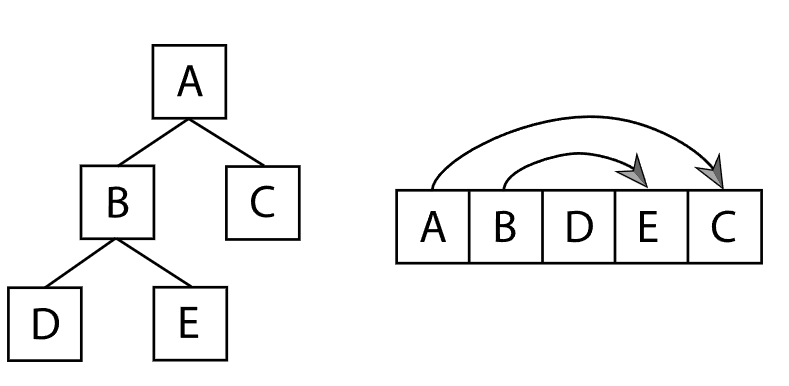
\includegraphics[width=8cm]{images/kdtree/compact.png}
     \caption{The compact representation of binary Kd-Tree in memory. The first child is discovered immediately after the parent node in memory. An offset pointer, illustrated here with lines and arrows, is used to locate the second child. The tree's leaf nodes (D, E, and C) have no children. \protect\cite{Pharr2016}}
        \label{fig:dice}
\end{figure}


\subsubsection{Surface Area Heuristic (SAH)}
Building a binary tree from top to bottom can be done using greedy \textbf{Surface Area Heuristics (SAH)}. The original scene is recursively partitioned using a greedy strategy for minimizing expected traversal cost. As the name suggested, this method of splitting nodes considers the area/volume of the primitives to find the splitting point.

\noindent
\\
Given a collection of $N$ primitives in a node tree with a total 3D volume $V$, and assuming that the split point chosen will partition the space into two halves $L$ and $R$ with several triangles $N_L$ and $N_R$, and corresponding volumes $V_L$ and $V_R$, respectively. With the previous configuration, the projected traversal cost can be approximated as:


\begin{equation}
Cost(V) = C_T + C_I(\frac{SA(V_L)}{SA(V)}N_L \frac{SA(V_R)}{SA(V)}N_R)
\end{equation}

\noindent
\\
Where: $V$: Total volume, $C_T$: Cost of traversal, $C_I$: Cost of intersection, $SA$: Surface area, $N$: Number of premitives, $•L$: Left, $R$: Right.

\noindent
\\
The following example visualizes and illustrates how the SAH works. Given a scene consisting of 7 primitives, we would like to find the best split using the SAH method. Because the intersection cost depends on the ray tracer implementation, we will set it to 1. In contrast, the estimated traversal cost was set to $\frac{1}{8}$. We will set the number of buckets to 8. The last numbers are chosen for more straightforward calculation only.

\noindent
\\
In the first iteration, the green colour represents the left space $L$, and the red colour represents the right space $R$. Since the example is 2D, the $SA $ equals the width multiplied by the rectangle's height. Each pixel has an area of 1. The SA of each rectangle is illustrated in Figure ~\ref{fig:sahdemo}. The overall surface area $SA(V)$ equals the summation of all the 7 primitives $1+1+4+4+4+1+1 = 16$. We can now substitute all the given information into the equation we get: 


\begin{align*}
& Cost\_iteration\_1 =  \frac{1}{8} + (\frac{1}{16}(1) +\frac{1+4+4+4+1+1}{16}(6)) = 5.81 \\
&Cost\_iteration\_2 =  \frac{1}{8} + (\frac{1+1}{16}(2) +\frac{4+4+4+1+1}{16}(5)) = 4.75 \\
&Cost\_iteration\_4 =  \frac{1}{8} + (\frac{1+1+4}{16}(3) +\frac{4+4+1+1}{16}(4)) = 3.75 \\
&Cost\_iteration\_7 =  \frac{1}{8} + (\frac{1+1+4+4+4+1}{16}(6) +\frac{1}{16}(1)) = 5.81 \\
\end{align*}


\noindent
\\
We choose the minimum cost. In the previous iterations, it is the 4th and then assigns the primitives on the left to the left node and the right primitives to the right node. Note that for simplicity, all primitives do not intersect. Unlike BVH, some primitives can be set to left and right if they are between the bucket's splitting point.


\begin{figure}[H]	
     \centering
     \begin{subfigure}[b]{0.475\textwidth}
         \centering
         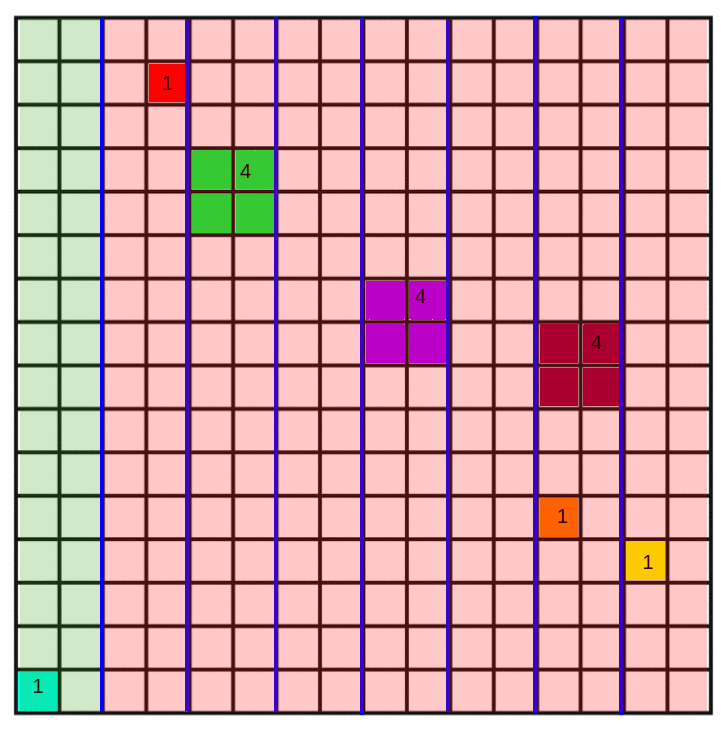
\includegraphics[width=5cm]{images/kdtree/grid_2.png}
         \caption{$1^{st} $ iteration.}
         \label{fig:pi_4000}
     \end{subfigure}
     \hfill
     \begin{subfigure}[b]{0.475\textwidth}
         \centering
         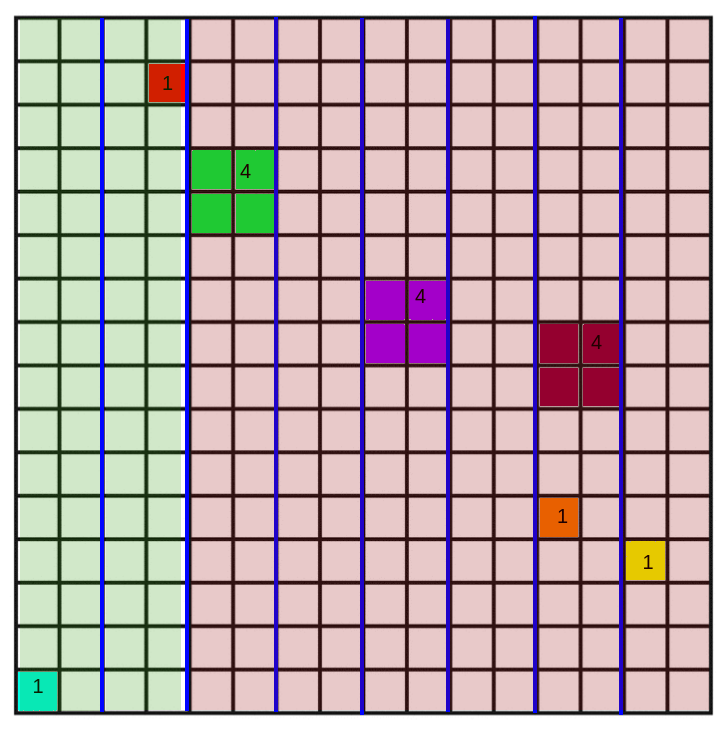
\includegraphics[width=5cm]{images/kdtree/grid_3.png}
         \caption{$2^{nd} $ iteration.}
         \label{fig:pi_5000}
     \end{subfigure}
     \hfill
     \begin{subfigure}[b]{0.475\textwidth}
         \centering
         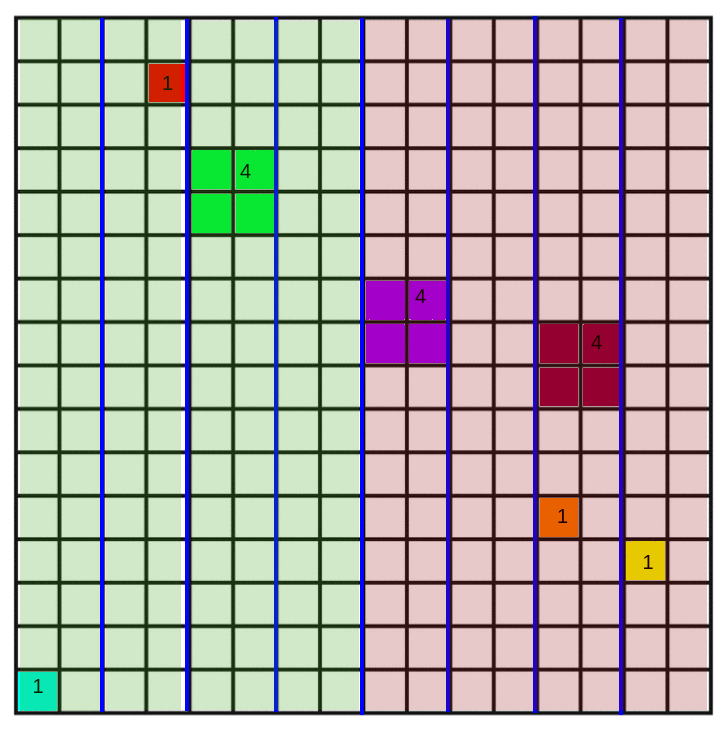
\includegraphics[width=5cm]{images/kdtree/grid_5.png}
         \caption{$4^{th} $ iteration.}
         \label{fig:pi_18000}
     \end{subfigure}
     \hfill
     \begin{subfigure}[b]{0.475\textwidth}
         \centering
         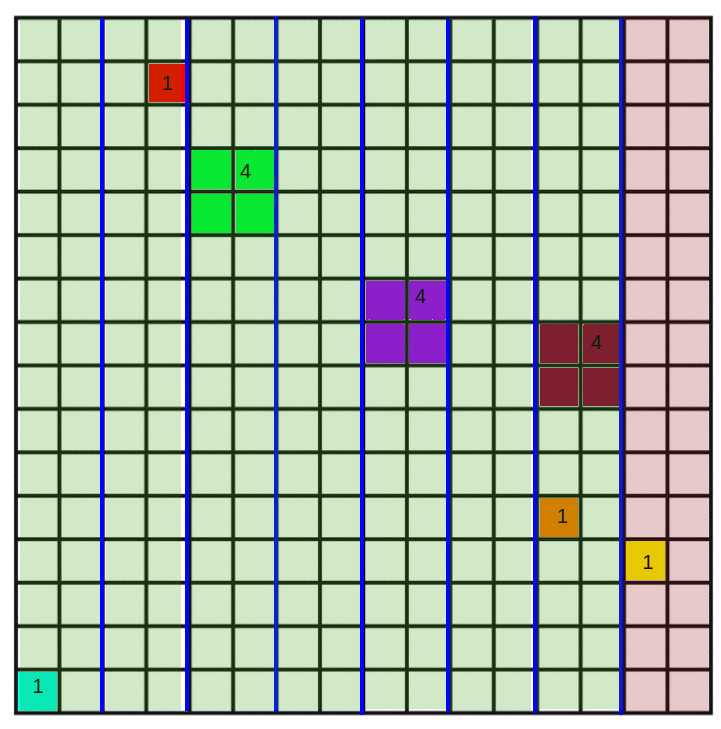
\includegraphics[width=5cm]{images/kdtree/grid_8.png}
         \caption{$7^{th} $ iteration.}
         \label{fig:pi_18000}
     \end{subfigure}
        \captionsetup{justification=centering,margin=2cm}
        \caption{Finding the best splitting point by using SAH. The left region is represented by green and the right region is represented by red.}
        \label{fig:sahdemo}
\end{figure}


\subsection{Implemntation}
The Kd-Tree has a variety of implementations, the one used in this project is based on \textbf{Physically Based Rendering PBR} \protect\cite{Pharr2016}. The implementation generates a binary tree that focuses on less memory consumption (Compact representation) and finds the best split by using the SAH method for splitting. We will be using a top-down approach as we did in BVH. We will split the implementation into two phases: Tree construction and tree traversal.

\noindent
\\
Kd-Tree is a variant of \textbf{Binary Space Partitioning (BSP)} tree. BSP trees use planes to divide the space into regions. It follows a top-down approach where a bounding box bounds the whole scene. If the number of primitives inside the bounding box exceeds a pre-defined parameter, we will name it \textit{maxPrims} then; the box is split into two sub-regions based on chosen splitting criteria. Each primitive is associated with the corresponding box/region that it intersects. Consequently, duplicated primitives can be assigned to more than one bounding box, unlike the BVH.

\noindent
\\
The procedure keeps repeating recursively until one of the two stop conditions occurs. Either the number of primitives in the sub-regions is less than \textit{maxPrims} or the other parameter, \textit{depth} is reached. The \textit{maxdepth} parameter is used to control the \textit{depth} of the tree.  

\noindent
\\
For simplicity and since AABB is used, only three axes will be considered for splitting x, y and z. However, this compromises some flexibility in how space is divided.

\subsubsection{Construction}
The recursive top-down algorithm is used to construct the Kd-Tree. We have a collection of primitives that overlap the axis-aligned space region at each step. Either the region is divided into two smaller ones and transformed into an inner node, or the recursion is stopped by making a leaf node out of the overlapping primitives.

\noindent
\\
In the Kd-Tree, we will save the nodes in an array and not in a tree representation, as mentioned before, to increase caching time. The issue is predetermining the number of nodes before building the tree to initiate the array. There are two approaches here. The first is to build the binary tree and then flatten it to an array (compact representation). The second approach is to allocate memory as we build the tree dynamically. The first approach needs two steps to build the tree and then transform it into a compact form, adding an extra step that reduces performance. Also, it consumes more memory as it needs to save the tree and adds an array that contains the same number of nodes as the tree. The latter approach is preferred as it consumes less memory and improves performance. However, it needs better handling for the memory allocation; this complexity depends on the implementation and the programming language used; therefore, the implementation will not be explained. 

\noindent
\\
For building the tree, the maximum allowed depth is needed to be given. However, what depth is preferred? Significant depth will increase the number of nodes, increasing memory consumption but reducing complexity from linear to more logarithmic. On the other hand, reducing the depth will decrease the number of nodes but will make the traversal time more linear, killing the use of the binary tree to reduce the complexity. A generic formula can be used to calculate the depth based on the \textbf{Physically Based Rendering PBR} \protect\cite{Pharr2016} book. This formula works for various scenes; $ N$ is the number of primitives in the scene, as the book suggests.



\begin{equation}
depth = 8 + 1.3\log(N)
\label{eq:depth}
\end{equation}

\noindent
\\
Since we are using memory allocation dynamically for the nodes array, each time the array is full, we will reallocate more memory double the size of the old array.

\noindent
\\
Unlike in the BVH, where we used the median point, in Kd-Tree, SAH is used to find the splitting point. The advantage of using median point is that it is intuitive to calculate and implement; nevertheless, it does not care about the area/volume of the primitive; it will simply split the primitives into two halves, unlike SAH, which considers the area/volume. Two parameters, $C_T$: Cost of traversal and $C_I$: Cost of intersection, are used in the SAH that will be tested and tweaked to find the best parameters. There are different methods to search for the best parameters for the best scenes; nevertheless, we will focus on the ratio between the two parameters instead. PBR suggests using 80 and 1, respectively.


\noindent
\\
One extra parameter, \textit{emptyBonus} denoted as $b_e$ will be added to the SAH algorithm. Since rays travelling through empty areas can progress to the next kd-tree node without having to do ray-primitive intersection checks, there is a little advantage for picking splits when one of the children has no primitives overlapping it. The parameter takes a value between 0 and 1 if one of the regions is empty and 0 otherwise. 



\begin{equation}
Cost(V) = C_T + (1-b_e)C_I(\frac{SA(V_L)}{SA(V)}N_L \frac{SA(V_R)}{SA(V)}N_R)
\end{equation}

\noindent
\\
One challenge left, if we want to consider all the splitting points as candidates, computing the cost of splitting is expensive, but as we mentioned before, we can use a fixed number of buckets. However, which is the best number for this parameter? The bigger the number, the more accurate the splitting point will be at the cost of building the tree's performance because more calculations are needed. Instead, we will only consider the limits of the bounding boxes. Hence we will need at most $2 * N$ buckets at each cost calculation, where $N$ is the number of primitives.

\begin{figure}[H]	
     \centering
     \captionsetup{justification=centering,margin=2cm}
     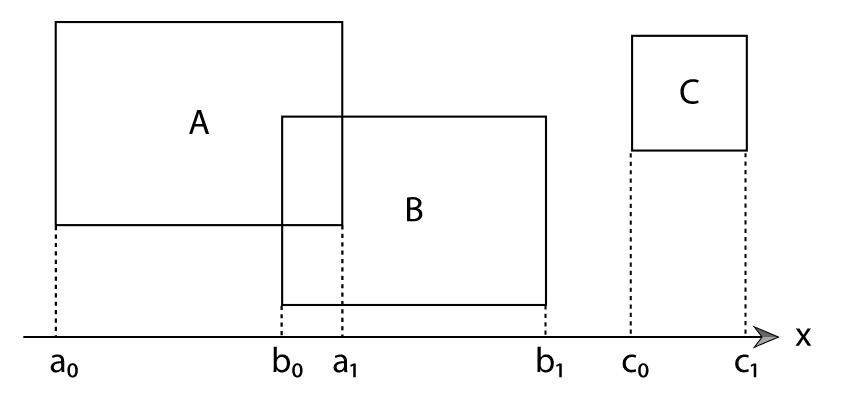
\includegraphics[width=10cm]{images/kdtree/projected_bboxes.png}
     \caption{Only six splitting points are considered. Taking $a_1$ as the splitting point will leave $A$ bounding box under it, $B$ overlapping it, and $C$ above it. \protect\cite{Pharr2016}}
        \label{fig:dice}
\end{figure}

\noindent
\\
Some edge cases can occur when the same number of primitives are assigned for both children. At this point, we are not gaining any performance from creating an interior node. The solution is to try other axes instead of the best-chosen axis. If the same edge case occurred for all axes, we would create one leaf node and assign all the primitives. It also can be worse to split than creating a leaf node based on the SAH algorithm. In that case, a leaf node is created rather than splitting. 

\subsubsection{Traversal}
The kd-Tree traversal is different from the BVH traversal we mentioned. BVH was a binary tree traversal where we start with the root node and go to the left or right child. On the other hand, the Kd-tree uses a depth-first, front-to-back traversal algorithm. 


\begin{figure}[H]	
     \centering
     \captionsetup{justification=centering,margin=2cm}
     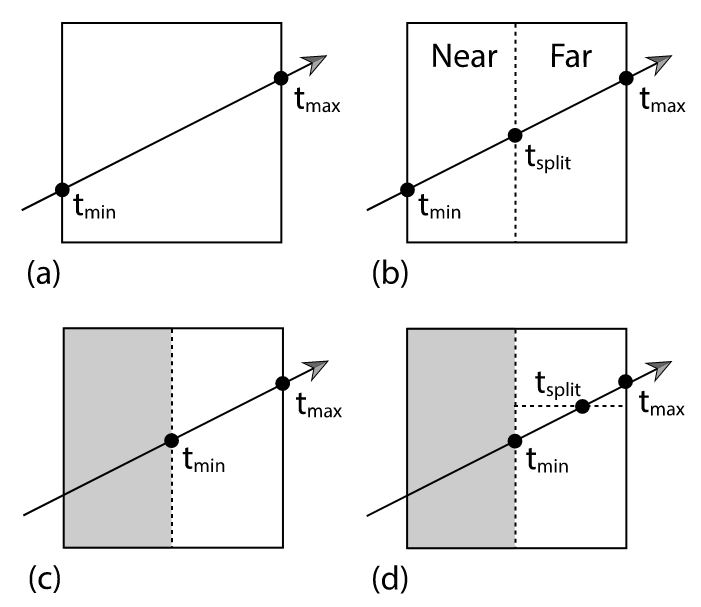
\includegraphics[width=10cm]{images/kdtree/traversal.png}
     \caption{(a) The initial intersection with the parent node, gives an initial parametric $[t_{min}, t_{max}]$ range to consider. (b) Because this range is nonempty, both children will be tested. The “near” node will be tested first where it has a parametric range $[t_{min}, t_{split}]$. If it is a leaf, its primitives will be tested; otherwise, its children will be tested recursively. (c) If the near node intersection test returns false, the far node will be tested. (d) Continuously keep visiting the tree nodes using depth-first, front-to-back traversal until the closest intersection is found or the ray exits the tree.  \protect\cite{Pharr2016}}
        \label{fig:dice}
\end{figure}

\noindent
\\
The first intersection test will start by testing if the ray intersects the global bounding box of the whole Kd-Tree $[t_{min}, t_{max}]$. If it returns false, we stop testing other nodes in the tree instantly because this means the ray does not pass any primitive.

\noindent
\\
If it returns true, we proceed to the next node using a depth-first, front-to-back traversal algorithm. If the next node is a leaf node, we iterate through the list of the primitives assigned to the node. As we discussed, we are not saving the primitives directly in the leaf node. We only save the number of primitives and the offset of the indices. It is a huge performance advantage, especially for the Kd-Tree, because in the Kd-Tree, one primitive can be in more than one node at a time. In terms of memory usage, if one leaf contains an N number of primitives, then there is a high chance of duplication of information with another leaf that contains these N primitives. It can be imagined with a million primitives. This can be at least twice the number of the original primitives. Before going through all the primitives, if the ray already intersected primitives in other nodes and those other nodes and the intersected point is less than the $t_{min}$ of the current node, then we are sure that we can not do better. We will not find any closer primitive in the leaf node. Hence we break and return. 
 

\noindent
\\
Otherwise, if it is an interior node, we would like to test its children, and unlike we did in the BVH, we were going left and right. This time we will use the intersection point to determine the left and right nodes. By comparing the splitting point with the intersected point, we can determine which children are more likely to be intersected first. This can be done quickly by checking if $t_{split} > t_{max}$, then we do not need to check the far child node (Second/Right node), same we check if $t_{split} < t_{min}$, then we do not check the near child node (First/Left node). Otherwise, we check them both by starting with the near (Left) and proceeding to the far (Right).   

\begin{figure}[H]	
     \centering
     \captionsetup{justification=centering,margin=2cm}
     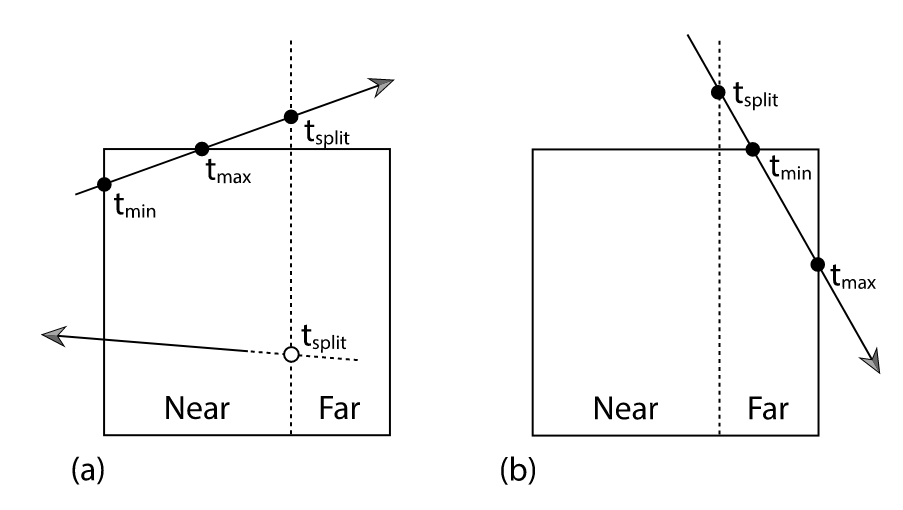
\includegraphics[width=10cm]{images/kdtree/traversal_case.png}
     \caption{Different scenarios prove the ray should not intersect both children. (a) The ray intersects the splitting plane at a point bigger than the $t_{max}$; hence we are sure it will not intersect the far child node. A negative sign denotes the bottom ray's direction away from the dividing plane. (b) Ray intersects the box at a point after the splitting plane, indicating that the near child is avoided.  \protect\cite{Pharr2016}}
        \label{fig:dice}
\end{figure}

\clearpage

\section{Performance Analysis}
 Optimizing parameters is part of rendering. Therefore, in this chapter, we will analyze the different data structures used, BVH, LBVH and Kd-Tree and how they perform against different scenes. We will pick up one data structure, Kd-Tree and tweak its different parameters and analyze how small changes in the parameter can affect the performance.


\noindent
\\
The following settings are used in this ray tracer:

\newcommand\T{\rule{0pt}{2.6ex}}       % Top strut
\newcommand\B{\rule[-1.2ex]{0pt}{0pt}} % Bottom strut

\begin{table}[H] 
\centering 
{\footnotesize
\begin{tabular}{ P{7cm} P{7cm} }      % centered columns (3 columns) 
\hline \hline
Property & Value \T\B  \\
\hline \hline
Machine & Intel(R) i7-8565U 16GB RAM\T\B
\\    
\hline
Resolution & 640x480  \T\B
\\
 \hline
Programming language & C++  \T\B 
\\ 
 \hline
Shading technique & Phong illumination \T\B 
\\
 \hline
\#Cameras & 1 \T\B 
\\
\#Lights & 1  \T\B 
\\ 
 \hline
 Models extention& .obj \T\B 
\\ 
 \hline
Anti-aliasing samples & 1 \T\B 
\\ 
\hline \hline
    \end{tabular}
}
  \caption{The settings used for the Ray tracer}
\end{table}

\subsection{How tweaking the data structure parameters affect performance}
Each data structure has its different implementation. In this subsection, we would like to illustrate how a slight change in each data structure parameter can produce different trees, affecting performance significantly. Only Kd-Tree will be investigated in terms of changing parameters and noticing their effect because the BVH and LBVH can do the same result, but they will be redundant.

\noindent
\\
Figure ~\ref{fig:kdtreeexample} shows two different constructed binary trees based on the same algorithm Kd-Tree and the same input scene; however, by changing the maximum number of primitives in the leaf node parameter \textit{maxPrims} from 1 to 2. We can note that one tree is shorter than the other! How would this affect the performance? 

\noindent
\\
A deeper tree means more nodes which leads to more memory consumption. Moreover, if the splitting criteria are too bad, this can lead to a long traversal time. On the other hand, a shallow tree can lead to fewer nodes but leaves that contain more primitives that will require a linear search (Brute force). 


\begin{figure}[H]	
     \centering
     \begin{subfigure}[b]{0.3\textwidth}
         \centering
         \captionsetup{justification=centering}
         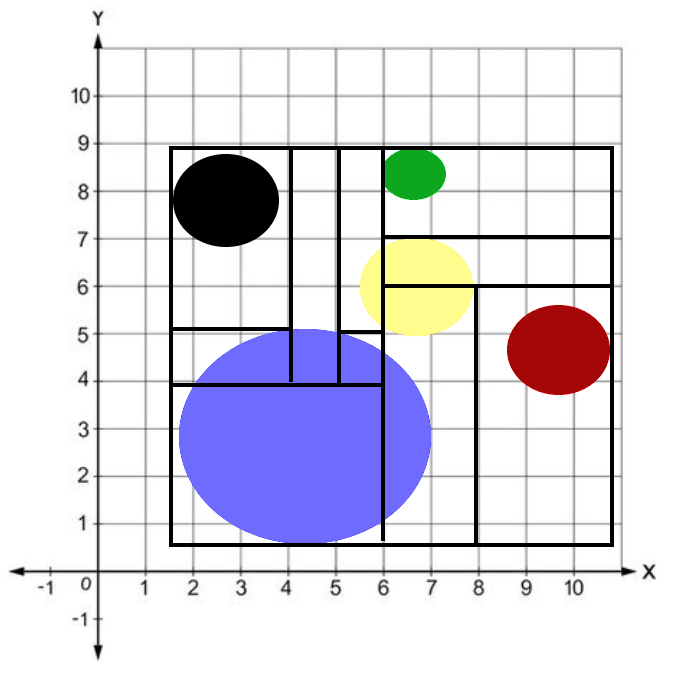
\includegraphics[width=\textwidth]{images/kdtree/visaul_scene_1_new.png}
         \caption{Kd-Tree generates regions (AABB) in a simple scene.}
         \label{fig:pi_4000}
     \end{subfigure}
     \hfill
     \begin{subfigure}[b]{0.6\textwidth}
         \centering
         \captionsetup{justification=centering}
         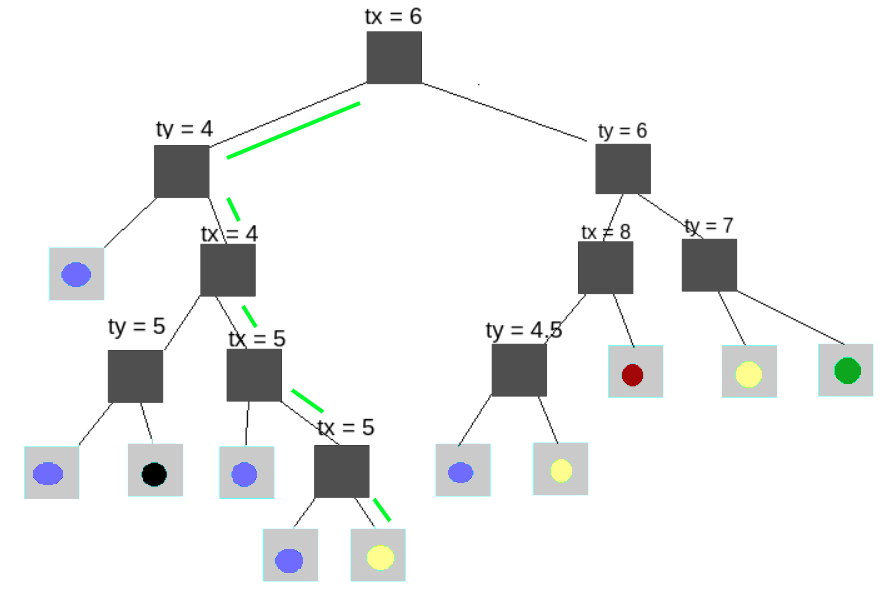
\includegraphics[width=\textwidth]{images/kdtree/visaul_tree_11_new.png}
         \caption{The resulting binary tree is based on the Kd-Tree algorithm with setting the maximum number of primitives in the leaf node parameter to 1.}
         \label{fig:kdtreeexampleb}
     \end{subfigure}
     \hfill
     \begin{subfigure}[b]{0.3\textwidth}
         \centering
         \captionsetup{justification=centering}
         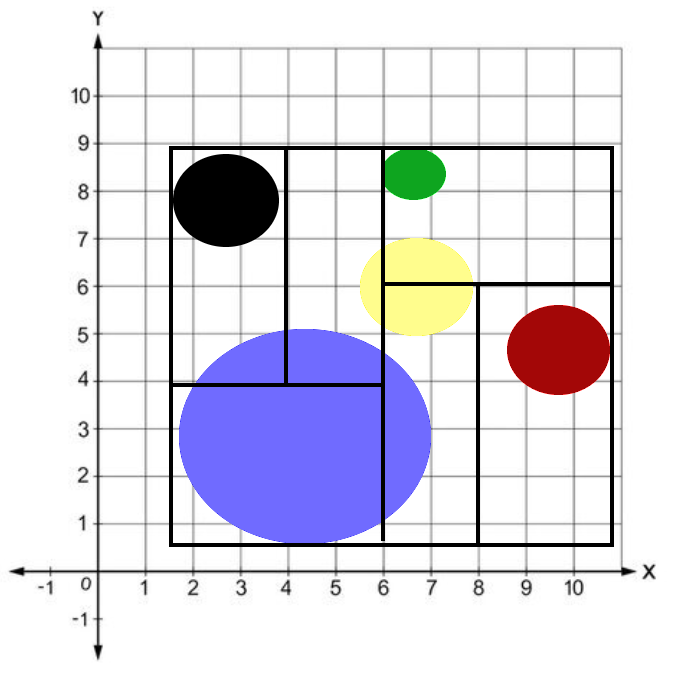
\includegraphics[width=\textwidth]{images/kdtree/visaul_scene_2_new.png}
         \caption{Kd-Tree generates regions (AABB) in a simple scene.}
         \label{fig:pi_5000}
     \end{subfigure}
     \hfill
     \begin{subfigure}[b]{0.6\textwidth}
         \centering
         \captionsetup{justification=centering}
         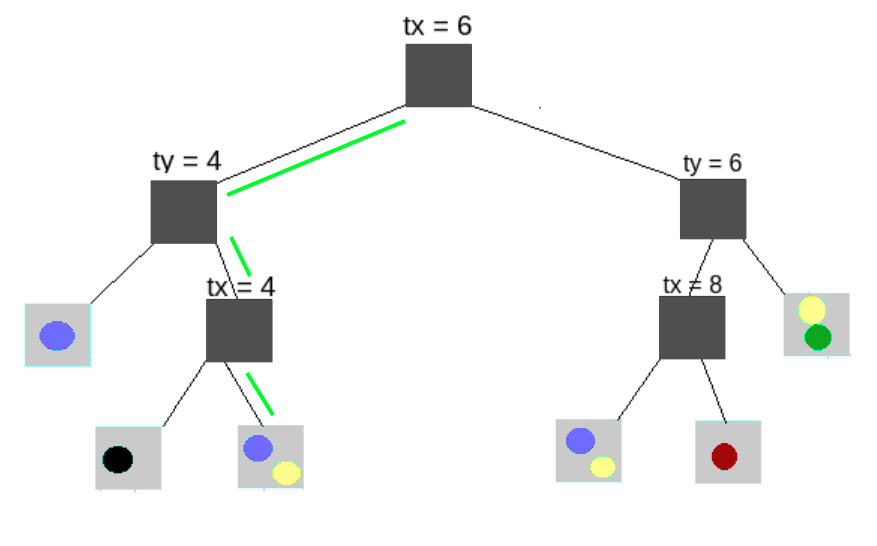
\includegraphics[width=\textwidth]{images/kdtree/visual_tree_2_new.png}
         \caption{The resulting binary tree is based on the Kd-Tree algorithm with setting the maximum number of primitives in the leaf node parameter to 2.
}
         \label{fig:kdtreeexampled}
     \end{subfigure}
        \captionsetup{justification=centering,margin=2cm}
        \caption{Two different constructed kd-trees with the same implementation and scene but with different parameters.}
        \label{fig:kdtreeexample}
\end{figure}

\noindent
\\
The next example demonstrates the performance differences between the two trees in simple math. Assuming the time consumed by the AABB intersection test is $0.1ms$. Let us calculate the time consumed to render the yellow sphere by talking the green path shown in the ~\ref{fig:kdtreeexample}. Sub-figure ~\ref{fig:kdtreeexampleb}
 needs five AABB tests resulting in $0.5ms$ to find the sphere, unlike in ~\ref{fig:kdtreeexampled}
 where only three AABB tests are needed resulting in $0.3ms$. The deeper tree has less performance than the other! Nonetheless, we did not consider the intersection cost of the spheres! In this example, the sphere intersection cost is tiny, but what if we replace the spheres with more complex models? Will the shallow tree still be better to use? In a shallow tree, the yellow sphere can be after the blue sphere in the list; hence one has to test the blue sphere first and then jump to the yellow. If the blue sphere (Model) generally has a high intersection cost, assumingly $0.3ms$. Then this will be added to the shallow tree cost to become $0.3ms + 0.3ms = 0.6ms$, which is larger than the long path in the deeper tree. Even though the model is as simple as a triangle or sphere only, we must remember that for the long list containing many primitives, this will add a leaner complexity.

\noindent
\\
After understanding the concept of the effect of the parameters on building the tree, Kd-Tree is used to analyse this further by using the current ray tracer. In this experience, we will change two parameters: The maximum number of primitives assigned to each leaf \textit{maxPrims} and the Maximum depth of the tree \textit{depth}. For better analyses, one model is fixed and used. Moreover, other SAH parameters are fixed to focus only on the two parameters mentioned. 

\noindent
\\
By changing the \textit{maxPrims} parameter and fixing the other parameters, we can note that the larger the value, the less it takes to build the tree. For instance, when increasing ${maxPrims}$ from  1 to 100, the build time increased by almost 2X. This is predictable; as we discussed before when the ${maxPrims}$ parameter is significant, we stop the recursion of building the tree; hence we stop creating more interior nodes; as shown in the table, the total number of nodes decreases by almost 418X. Consequently, the tree depth becomes smaller. On the other hand, we note that rendering time increased by 1.2X. This is because some leaf contains 100 primitives that the ray has to go through them linearly and test them until it finds the right primitive or, even worse, not find an intersection after going through 100 primitive intersections. This explains why the number of intersection tests shown in the table has increased by almost  61X. Setting the value to 10 as a trade-off results in an acceptable building and the rendering time.


\begin{table}[ht] 
\centering 
{\footnotesize
\begin{tabular}{ P{2.5cm} ||P{2.1cm}  P{2.1cm}  P{2.1cm} P{2.1cm}  P{2.1cm}}      % centered columns (3 columns) 
\hline\hline                                      %inserts double horizontal lines
\Includegraphics[height=1in]{images/stanford-bunny-black.png}
& \#Primitives  & \#Nodes & \#Primitives intersection tests & Build(s) & Render(s) \\ [0.5ex] % inserts table heading 
\hline
    \end{tabular}
}
\end{table}
\vspace{-2em}
\begin{table}[ht] 
\centering 
{\footnotesize
\begin{tabular}{ P{2.5cm} ||P{2.1cm}  P{2.1cm}  P{2.1cm} P{2.1cm}  P{2.1cm} }      % centered columns (3 columns) 
 \hline
maxPrims = 1& 35, 947 & 418, 548 & 192, 171 &  5.214 s & 20.845 s\T\B 
\\ 
maxPrims = 10& 35, 947 & 19, 229 & 1, 381, 296 & 2.033 s & 20.211 s
\T\B 
\\ 
maxPrims = 100& 35, 947 & 1, 461 & 11, 761, 329 & 2.865 s & 24.062 s\T\B 
\\ 
\hline \hline
depth = 5 & 35, 947 & 61 & 140, 964, 745 &  0.7 s & 37.762 s \T\B 
\\ 
depth = 10& 35, 947 & 1, 435 & 10, 571, 611 & 1.239 s & 11.566 s\T\B 
\\ 
depth = 28& 35, 947 & 44, 852 & 683, 669 & 1.757 s & 9.606 s\T\B 
\\ 
depth = 100& 35, 947 & 44, 854 & 683, 669 & 1.871 s & 9.546 s\T\B 
\\ 
\hline \hline
    \end{tabular}
}
  \captionsetup{justification=centering,margin=2cm}
  \caption{Changing Kd-Tree parameters and how they affect performance by using \protect\cite{stanfordbunny}}
\end{table}

\noindent
\\
Increasing the number of the depth parameter increases the building time; however, it reduces the rendering time significantly. For example, by changing the depth from 5 to 10, the building and rendering time combined is reduced by almost 3X. Although the building time is increased, we notice the massive gain in the rendering time, which is very often the bottleneck in ray tracing. By changing the value from 10 to 28, which is the value suggested by the Equation \eqref{eq:depth} we mentioned earlier, we note that the overall performance increased by almost 1.2X. Increasing the depth to 100 reaches a saturation point where the depth does not play any role in performance. The reason is that for each scene, there is a maximum value depth that the tree can produce, and regardless of increasing the depth parameter, if the parameter is more significant than the maximum depth of the tree, then it is useless to constrain the tree with the value more significant than its maximum reachable depth. We can conclude that the formula used in the PBR book looks promising and delivers the best result from the values used in the table. 

\noindent
\\
Tweaking both parameters to find the optimal result is different from tweaking one parameter and fixing one. In order to find the best combination of parameters for a random scene, one can use one of the well-known parameter optimization techniques such as  Grid Search. Parameter optimization techniques will not be covered in this report.  


\subsection{Investigating different data structures}
Different models with a diverse range of primitives are used for proper comparison. The models Stanford-bunny \protect\cite{stanfordbunny}, Igea \protect\cite{igea}, Asian Dragon \protect\cite{stanfordxyzdragon}, and Happy Buddha \protect\cite{buddha} used are taken from the following repository \protect\cite{Jacobson2021}.

\noindent
\\
Useful metrics have been calculated for the three mentioned data structures against different models. Since each data structure needs a pre-processing time to be constructed and built, \textit{(build)} time in seconds corresponds to how many seconds each data structure took to be ready to be used for the rendering stage. Rendering time \textit{(render)} is also essential to measure, as it indicates how long the overall rays travelled through the scene and includes the traversal phase. The number of intersection tests \textit{(\#int. tests)} done for the primitives is also crucial as it explains how many intersection tests are done in the rendering phase. Usually, less number of intersection tests indicates better performance. The total number of nodes metric \textit{(\#nodes)} indicates the complexity of the constructed tree and how deep it is. 

\noindent
\\
Since each data structure is built using different parameters, we will fix the parameters and only change scenes. The following table shows the settings for each data structure.

\begin{table}[H] 
\centering 
{\footnotesize
\begin{tabular}{ P{7cm} P{7cm} }      % centered columns (3 columns) 
\hline \hline
Data structure & Parameters \T\B  \\
\hline \hline
BVH & $depth=50,\; maxPrims=1,\; splitting=median$\T\B
\\    
\hline
LBVH & $depth=50,\; maxPrims=1,\; splitting=morton code$ \T\B
\\
 \hline
Kd-Tree & $depth = 8 + 1.3\log(N),\; maxPrims=1,\; splitting=SAH$ \T\B 
\\ 
\hline \hline
    \end{tabular}
}
  \caption{Parameters used for each data structure}
\end{table}

\noindent
\\
Considering the building time metric. We note that BVH is the fastest to build the tree, and Kd-Tree is the slowest; nonetheless, LBVH stays in the middle. BVH is the fastest because it uses simple splitting criteria, which is the median of the primitives. This is a cheap performance execution. Moreover, it uses a simple tree representation and does not use a compact form as Kd-Tree. LBVH is almost 2X of the BVH; even though both use the same binary tree, the splitting criteria are different. LBVH has to map the centre point of the 3D primitive to a Morton code, sort it by radix sort and then find a splitting point. These extra three stages add extra complexity to the building phase. Hence LBVH takes more time than BVH for this implementation. Kd-Tree consumes much time in the building phase since it uses the SAH algorithm to split nodes. As we explained already with an example, the SAH method can be expensive to compute, especially for some edge cases where the splitting point can not be found, and the algorithm tries the three different axes until it finds the best split or just split the AABB into halves. 

\noindent
\\
The second metric is the rendering time. BVH and LBVH have similar rendering performances because both use the same tree traversal algorithm (Pre-order Traversal). By adding both building and rendering time, we can note that BVH spends less time than LBVH. We conclude that in the current implementation, BVH outperforms LBVH. LBVH is primarily beneficial during construction as the tree can be built on multi threads. However, this is not included as it is intuitive that multithreading will increase any algorithm performance. Multithreading LBVH can construct the tree faster than BVH, and since both are similar in rendering time, LBVH can outperform BVH in that scenario. On the other hand, Kd-Tree spends less time on the smaller models with few primitives than the ones with 1 million primitives. Adding both buildings to the rendering time, we note that Kd-Tree consumes much more time than the other data structures due to its expensive building time. 



\begin{table}[H] 
\centering 
{\footnotesize
\begin{tabular}{ P{2.5cm}||P{2.5cm}P{2.5cm} P{2.5cm} P{2.5cm}  }      % centered columns (3 columns) 
\hline\hline                                      %inserts double horizontal lines
Model name& Stanford-bunny  & Igea & Asian Dragon & Happy Buddha \\ [0.5ex] % inserts table heading 
\hline\hline 
Model image
&
\Includegraphics[height=1in]{images/stanford-bunny-black.png}& \Includegraphics[height=1in]{images/igea-black.png} & \Includegraphics[height=1in]{images/xyzrgb_dragon.png} & \Includegraphics[height=1in]{images/happy-black.png} \\

\hline \hline
\#Primitives & 35, 947  & 134, 345 & 539, 205 & 1, 078, 410 \T\B
\\
\hline \hline
BVH build(s)& 0.849 s& 2.739 s & 21.105 s & 34.687 s \T\B 
\\ 
LBVH build(s)& 1.272 s& 4.401 s & 45.98 s & 58.234 s \T\B 
\\
Kd-Tree build(s)& 2.346 s& 30.075 s & 120.078 s & 211.078 s \T\B 
\\
\hline \hline
BVH render(s)& 17.707 s& 13.986 s & 41.588 s & 51.516 s \T\B 
\\
LBVH render(s)& 11.512 s& 13.796 s & 40.744 s & 51.14 s \T\B 
\\
Kd-Tree render(s)& 9.405 s& 12.111 s & 45.292 s & 34.292 s \T\B 
\\
\hline \hline
BVH \#int. tests & 139, 926 & 365, 715  & 2, 429, 951  & 3, 279, 593  \T\B 
\\
LBVH \#int. tests & 93, 641 & 365, 712  & 2, 429, 942  & 3, 279, 593  \T\B 
\\
Kd-Tree \#int. tests & 128, 943 & 74, 516  & 483, 710  & 943, 201  \T\B 
\\
\hline \hline
BVH \#nodes & 71, 893 & 268, 689  & 1, 078, 409  & 2, 156, 819  \T\B 
\\
LBVH \#nodes & 71, 889 & 268, 669  & 1, 077, 768  & 2, 156, 352  \T\B 
\\
Kd-Tree \#nodes & 418, 661 & 2, 830, 597  & 415, 406  & 375, 243  \T\B 
\\
\hline \hline

    \end{tabular}
}
\captionsetup{justification=centering,margin=2cm}
\caption{Comparison between BVH, LBVH and Kd-Tree by using different models \protect\cite{stanfordbunny}, \protect\cite{igea}, \protect\cite{stanfordxyzdragon}, \protect\cite{buddha}}
\end{table}
\noindent
\\
Concerning the number of nodes and intersections, one can note that BVH and LBVH generally deliver approximately similar output. The built tree for both methods may be due to some similarity in the splitting criteria as the median method is equivalent to the Morton code. It is only a conclusion I made. Kd-Tree shows a more complex tree representation for the smaller model and a simple tree for the larger models. Because the SAH algorithm can produce duplicated primitives in different nodes leading to long deep trees and more nodes, on the other hand, for bigger models, the number of nodes and intersections is reduced significantly. Spending more time to construct and optimise the tree will lead to longer building time; however, it acts as an investment to produce a better tree to boost the rendering (traversal) time.


\noindent
\\
Although the average performance correlates to the number of primitives in the scene, some small scenes produce complex trees and considerable building time. For instance, looking at the Kd-Tree number of nodes can spike up because not only is the number of primitives vital to choosing the proper data structure, but other perspectives related to the scene can affect the performance, not only the number of primitives. The following scenes try to cover some of them.

\noindent
\\
\subsection{Investigating much more complex scenes}

\begin{table}[H] 
\centering 
{\footnotesize
\begin{tabular}{ P{2.5cm}||P{5cm}P{5cm} }      % centered columns (3 columns) 
\hline\hline                                      %inserts double horizontal lines
Model name& Trees & Sci-Fi Tropical City   \T\B 
\\
\hline\hline 

Model image&
\Includegraphics[width=5cm]{images/tree.png}
& \Includegraphics[width=5cm]{images/SCIFI.png}
\\

\hline \hline
\\
\#Primitives & 252, 178  & 90, 811\\ [0.5ex] % inserts table heading 
\\
\hline \hline
BVH build(s)& 4.373 s& 1.556 s\T\B
\\
LBVH build(s)& 12.062 s& 5.408 s \T\B
\\
Kd-Tree build(s)& 55.325 s& 14.164 s \T\B
\\
\hline \hline
BVH render(s)& 42.028 s& 54.690 s \T\B
\\
LBVH render(s)& 39.330 s& 49.636 s \T\B
\\
Kd-Tree render(s)& 22.822 s& 25.705 s  \T\B
\\
\hline \hline
BVH \#int. tests & 907, 969 & 1, 250, 079  \T\B
\\
LBVH \#int. tests & 914, 992 & 1, 031, 416  \T\B
\\
Kd-Tree \#int. tests & 4, 486, 021 & 2, 813, 475  \T\B
\\
\hline \hline
BVH \#nodes & 131, 047 & 65, 535 \T\B
\\
LBVH \#nodes & 131, 038 & 65, 530 \T\B
\\
Kd-Tree \#nodes & 511, 023 & 272, 881 \T\B
\\
\hline \hline

    \end{tabular}
}
\end{table}
\subsubsection{Trees}
Special thanks to \protect\cite{trees} for the Trees 3D model. This scene has a high discrepancy, where some primitives create clusters at regions such as the trees' leaf where there is a compact number of primitives but with some empty spaces between them. On the other hand, there is the ground, the sky, which is an empty region. Note that this scene uses textures but is turned off in the current ray tracer. 


\noindent
\\
Looking at the result, we can note that LBVH and BVH are still delivering almost the same result. Even though the building and rendering times differ, the overall performance is relatively close. The number of generated nodes is similar. Kd-Tree consumes more than double the time to construct the tree, generating almost 4.5 million nodes which are almost 4.5X in BVH and LBVH. However, the rendering time is almost half because Kd-Tree allows the same primitives to be in more than one node leading to duplication, more nodes, and a deeper binary tree. 

\noindent
\\
The Kd-Tree outperformed BVH and LBVH in rendering time by more than 2X. Even though it was previously tested on Igea and the Asian Dragon models, it did not outperform the other data structures. Although the number of Trees scene 252K primitives is between 134k and 539K, the result we expect to be in between or at least the Kd-Tree still suffering, but this was not the result. This scene hints at how different data structures can perform differently based on the number of primitives and the distribution of primitives. The difference between the Trees scene and other models tested is that the Trees scene consists of a dense cluster of primitives, the Trees leaves, and other regions where no primitives exist (Sky and Floor). We can note that kd-Tree, combined with SAH, performs better with sich scenes. 


\subsubsection{Sci-Fi Tropical City}
Special thanks to \protect\cite{scifi} for the Sci-Fi Tropical City 3D model. Although this scene has fewer primitives than the Trees scene, it has more details. The same result for both BVH and LBVH where BVH outperformed LBVH in the building time, but LBVH outperformed BVH in rendering time, but the overall time is almost similar. Both of them did not perform well. We note that both rendering time is more than the rendering time for rendering the Igea model, which was 134k. Both took 13s to render for the Igea model, whereas for the Sci-Fi, it took around 50s. This is because this scene is more detailed and covers most of the projected plane. Kd-Tree furthermore outperformed both BVH and LBVH in the rendering time. Interestingly the number of nodes is less than nodes generated in the Stanford bunny, which was more than the 3x number of the Sci-fi scene. We note that even though the number of intersections is 21X of the intersections test in the Stanford bunny, we expect the rendering time to be significantly higher; however, it increased only by 2.6X. 



\noindent
\\
\clearpage

\section{Conclusion}
In this report, we started discussing how significant the impact of acceleration structures is on ray tracing. We explained two types of data structures, object subdivision types such as BVH and LBVH and spacial subdivision such as Kd-Tree. Each method consists of two major phases Construction tree and the Traversal tree. Each technique uses different parameters that can be tweaked, resulting in different trees that lead to different building and rendering times. Splitting criteria play an essential role in how to produce a decent tree. A decent tree means a tradeoff between the depth of the tree and the number of primitives assigned to each leaf node.  

\noindent
\\
BVH outperformed LBVH and Kd-Tree in building the tree time in most scenes. This is due to its simple splitting criteria where it only divides the primitives into two halves. LBVH, on the other hand, took more time to build the tree due to its Morton code generation and radix sorting algorithm. Although LBVH makes it easier to build sub trees independently from each other, the rendering time for both LBVH and BVH was quite similar in most scenes. This is because both methods use pre-order traversal methods and generate a similar number of nodes.

\noindent
\\
Kd-Tree invests much more time building the tree because it uses the SAH algorithm. Moreover, Kd-Tree allows duplicated primitives in more than one node, resulting in deeper trees than BVH and LBVH. This is noticeable by looking at the number of nodes generated. However, Kd-Tree spend less time on rendering than other methods; this is critical for complex scenes such as Trees and Sci-Fi. For small models, we note that it is acceptable to use BVH and LBVH.

\noindent
\\
Data structures produce different results depending on the scene, implementation, and chosen parameters. Some implementation uses more than one data structure on different models in the scene. Moreover, different bounding volumes can be chosen, not only fixing it to AABB. There is no clear winner. Each implementation has pros and cons; nevertheless, one can tweak the parameters to optimize the performance depending on the scene.


\noindent
\\
The author thanks his supervisor \textbf{Prof.Dr.-Ing. Matthias Teschner} once again for the guidance throughout this project.
	
\clearpage

\bibliographystyle{apacite}
\bibliography{References}

\end{document}
